\documentclass[11pt, aspectratio=169]{beamer}

\usepackage{amsmath, amsfonts, microtype, nicefrac, amssymb, amsthm, centernot}

\usepackage{pgfpages}

\usepackage{helvet}
\usepackage[default]{lato}
\usepackage{array}

\usefonttheme[onlymath]{serif}

\usepackage[utf8]{inputenc}
\usepackage[T1]{fontenc}
\usepackage{textcomp}
\usepackage{bm}

\usepackage{mathpazo}
\usepackage{hyperref}
\usepackage{multimedia}
\usepackage{graphicx}
\usepackage{multirow}
\usepackage{graphicx}
\usepackage{dcolumn}
\usepackage{bbm}
\newcolumntype{d}[0]{D{.}{.}{5}}

\usepackage{graphicx}
\usepackage[space]{grffile}
\usepackage{booktabs}

\usepackage{setspace}

\usepackage{transparent}


%%% FIGURES %%%
\usepackage{caption, subcaption}
\usepackage{booktabs, siunitx}
\usepackage{pgfplots} 
%\usepackage[outdir=./figures]{epstopdf}
\usepackage{float}
\usepackage{graphicx}
\usepackage[absolute, overlay]{textpos}
\usepackage{epstopdf}


%%% TIKZ %%%
\usepackage{tikz}
\usepackage{verbatim}
\usetikzlibrary{arrows.meta}
\usetikzlibrary{positioning}
\usetikzlibrary{bending}
\usetikzlibrary{snakes}
\usetikzlibrary{calc}
\usetikzlibrary{arrows}
\usetikzlibrary{decorations.markings}
\usetikzlibrary{shapes.misc}
\usetikzlibrary{matrix, shapes, arrows, fit, tikzmark}


%%% ALGORITHM %%%
\usepackage{algorithm}
\usepackage[noend]{algpseudocode}
\usepackage{multimedia}


%%% APPENDIX SLIDE NUMBERING %%%
\usepackage{appendixnumberbeamer}


%%% BEAMER BUTTON %%%
%\setbeamertemplate{button}{\tikz
	%\node[
	%	inner xsep = 2pt, 
	%	draw = structure!0, 
	%	fill = myblue, 
	%	rounded corners = 4pt]{\color{white} \tiny\insertbuttontext};
	%}


%%% COLORS %%%
\definecolor{blue}{RGB}{0,38,118}
\definecolor{red}{RGB}{213,94,0}
\definecolor{yellow}{RGB}{240,228,66}
\definecolor{green}{RGB}{0,158,115}

\definecolor{myred}{RGB}{163,32,45}
\definecolor{navyblue}{rgb}{0.05,0.2,0.70}
\definecolor{myblue}{RGB}{0,51,150}
\definecolor{myorange}{RGB}{255,140,0}
\definecolor{myref}{RGB}{160,160,160}
\definecolor{shock}{RGB}{0, 125, 34}%{50, 168, 82}

\definecolor{background}{RGB}{255,253,218}

% Define a new transparent color
\definecolor{trans}{rgb}{1,1,1}
\colorlet{trans}{black!20} % 0 percent opacity

\hypersetup{
  colorlinks=false,
  linkbordercolor = {white},
  linkcolor = {blue}
}

\setbeamercolor{frametitle}{fg=blue}
\setbeamercolor{title}{fg=black}
\setbeamertemplate{footline}[frame number]
\setbeamertemplate{navigation symbols}{} 
\setbeamertemplate{itemize items}{-}
\setbeamercolor{itemize item}{fg=blue}
\setbeamercolor{itemize subitem}{fg=blue}
\setbeamercolor{enumerate item}{fg=blue}
\setbeamercolor{enumerate subitem}{fg=blue}
\setbeamercolor{button}{bg=background, fg=blue,}

%\setbeamercolor{background canvas}{bg=background}


%%% FRAME TITLE %%%
\setbeamerfont{title}{series=\bfseries, parent=structure}
\setbeamerfont{frametitle}{series=\bfseries, parent=structure}


%%% TRANSITION FRAME %%%
\newenvironment{transitionframe}{
	\setbeamercolor{background canvas}{bg=blue}
	\begin{frame}
		\thispagestyle{empty}
		\addtocounter{framenumber}{-1}
		\vspace{42mm}
		\hspace{4mm} }{
		\begin{tikzpicture}
			\tikz \fill [white] (1,6) rectangle (20,10);
		\end{tikzpicture}
	\end{frame}
}


%%% OUTLINE %%%
\AtBeginSection[]
{
	\begin{frame}
       \frametitle{Roadmap of Talk}
       \tableofcontents[currentsection]
   \end{frame}
}
\setbeamercolor{section in toc}{fg=blue}
\setbeamercolor{subsection in toc}{fg=red}
\setbeamersize{text margin left=1em,text margin right=1em} 


%%% ENVIRONMENTS
\newenvironment{witemize}{\itemize\addtolength{\itemsep}{10pt}}{\enditemize}

\makeatother
\setbeamertemplate{itemize items}{\large\raisebox{0mm}{\textbullet}}
\setbeamertemplate{itemize subitem}{\footnotesize\raisebox{0.15ex}{--}}
\setbeamertemplate{itemize subsubitem}{\Tiny\raisebox{0.7ex}{$\blacktriangleright$}}

\setbeamertemplate{enumerate item}[default]
\setbeamertemplate{enumerate subitem}{\textbullet}
\makeatletter

% ITEMIZE SPACING:
% \usepackage{xpatch}
% \xpatchcmd{\itemize}
% {\def\makelabel}
% {\setlength{\itemsep}{0mm}\def\makelabel}
% {}
% {}


%%% PRETTY ENUMERATE %%%
% \usepackage{stackengine,xcolor}
% \newcommand\circnum[2]{\stackinset{c}{}{c}{.1ex}{\small\textcolor{white}{#2}}%
	% 	{\abovebaseline[-.7ex]{\Huge\textcolor{#1}{$\bullet$}}}}
% \newenvironment{myenum}
% {\let\svitem\item
	% 	\renewcommand\item[1][black]{%
		% 		\refstepcounter{enumi}\svitem[\circnum{##1}{\theenumi}]}%
	% 	\begin{enumerate}}{\end{enumerate}}
\usepackage{stackengine,xcolor,graphicx}
\newcommand\circnum[2]{\smash{\stackinset{c}{}{c}{.2ex}{\small\textcolor{white}{#2}}%
		{\abovebaseline[-1.1ex]{\Huge\textcolor{#1}{\scalebox{1.5}{$\bullet$}}}}}}
\newenvironment{myenum}
{\let\svitem\item
	\renewcommand\item[1][black]{%
		\refstepcounter{enumi}\svitem[\circnum{##1}{\theenumi}]}%
	\begin{enumerate}}{\end{enumerate}}

\newcommand{\notimplies}{\;\not\!\!\!\implies}


%%% BEN'S SHORTCUTS %%%
\newcommand{\bi}{\begin{itemize}}
\newcommand{\ei}{\end{itemize}}
\newcommand{\be}{\begin{enumerate}}
\newcommand{\ee}{\end{enumerate}}
\newcommand{\bd}{\begin{description}}
\newcommand{\ed}{\end{description}}
\definecolor{gred}{RGB}{200,0,25}
\definecolor{gblue}{RGB}{25,0,200}
\definecolor{ggreen}{RGB}{25,200,25}
\definecolor{dgreen}{rgb}{0,0.5,0}
\definecolor{gpink}{RGB}{255,0,247}

\definecolor{foreground}{RGB}{0,0,0}
\definecolor{background}{RGB}{255,255,255}
%\definecolor{title}{RGB}{37,47,141}
\definecolor{title}{RGB}{0,0,0}
%\definecolor{title}{RGB}{25,0,200}
\definecolor{gray}{RGB}{155,155,155}
%\definecolor{subtitle}{RGB}{128,128,128}
\definecolor{subtitle}{RGB}{0,0,0}
\definecolor{hilight}{RGB}{102,255,204}
\definecolor{vhilight}{RGB}{255,111,207}

\newtheorem{assumption}{Assumption}
\newtheorem{condition}{Condition}
\newcommand{\tw}{\textcolor{white} }
\newcommand{\tblk}{\textcolor{black} }
\newcommand{\tr}{\textcolor{gred} }
\newcommand{\tb}{\textcolor{gblue} }
\newcommand{\tg}{\textcolor{dgreen} }
\newcommand{\tp}{\textcolor{gpink} }

\usepackage{ushort}



%%%%%%%%%%%%%%%%%%%%%%%%%%  TITLE   %%%%%%%%%%%%%%%%%%%%%%%%%%%%%%%%
\title[]{\\[8pt]
	{\large \color{blue} Dynamic Programming and Applications \\[5pt] \normalfont{Heterogeneous Agents and Inequality} \\[10pt] \normalfont{Lecture 10}}}
\author[Schaab]{Andreas Schaab}
\institute{}
\subject{}
\date{}



%%%%%%%%%%%%%%%%%%%%%%%%  BEGIN DOC   %%%%%%%%%%%%%%%%%%%%%%%%%%%%%%%
\begin{document}

%%% TIKZ %%% 
\tikzstyle{every picture}+=[remember picture]
%\everymath{\displaystyle}

\tikzset{   
	every picture/.style={remember picture,baseline},
	every node/.style={anchor=base,align=center,outer sep=1.5pt},
	every path/.style={thick},
}
\newcommand\marktopleft[1]{%
	\tikz[overlay,remember picture] 
	\node (marker-#1-a) at (-.3em,.3em) {};%
}
\newcommand\markbottomright[2]{%
	\tikz[overlay,remember picture] 
	\node (marker-#1-b) at (0em,0em) {};%
}
\tikzstyle{every picture}+=[remember picture] 
\tikzstyle{mybox} =[draw=black, very thick, rectangle, inner sep=10pt, inner ysep=20pt]
\tikzstyle{fancytitle} =[draw=black,fill=red, text=white]


\addtocounter{framenumber}{-1}
\thispagestyle{empty}
\maketitle 
\newpage

%%%%%%%%%%%%%%%%%%%%%%%%%%  SLIDE   %%%%%%%%%%%%%%%%%%%%%%%%%%%%%%%%
\begin{frame}{What this part of the course is about}
\begin{witemize}
\item Understanding \textbf{cross-sectional household heterogeneity} (``inequality'') is one of the biggest questions in macroeconomics 

\item Vast literature studies and models inequality since at least 1980s

\item First wave of research: document inequality and understand where it comes from

\item Recent ``boom'' in \textbf{heterogeneous agent macro}: inequality shapes aggregate outcomes (business cycles, growth, policy transmission, ...)
\end{witemize}
\end{frame}

%%%%%%%%%%%%%%%%%%%%%%%%%%  SLIDE   %%%%%%%%%%%%%%%%%%%%%%%%%%%%%%%%
\begin{frame}{Heterogeneous agent models}

\begin{witemize}
\item Studying inequality (both its origins and consequences) requires modeling \textbf{distributions}

\item This is very difficult because distributions are large, high-dimensional objects

\item But also opens door to vast number of interesting questions:
\begin{itemize}
\item Why are income and wealth so unequally distributed? What explains changes over time?
\item Is there a trade-off between inequality and economic growth?
\item How does inequality vary over the business cycle?
\item Does inequality affect the transmission and effectiveness of monetary and fiscal policy?
\end{itemize}

\item Main idea: solving heterogeneous agent models = solving PDEs

	{\footnotesize This is the current frontier in macro. This is why we invested so much in studying differential equations!}
\end{witemize}
\end{frame}


%%%%%%%%%%%%%%%%%%%%%%%%%%  SLIDE   %%%%%%%%%%%%%%%%%%%%%%%%%%%%%%%%
\begin{frame}{Solving HA models = solving PDEs}

\vspace{2mm}
\begin{witemize}
\item More precisely: a system of two PDEs
\begin{enumerate}
	\item {\color{blue}\textbf{Hamilton-Jacobi-Bellman}} equation for individual choices
	\item {\color{blue}\textbf{Kolmogorov Forward}} equation for evolution of distribution
\end{enumerate}

\item Many well-developed methods for analyzing and solving these \\
{\footnotesize \url{https://benjaminmoll.com/codes/}}
\\
{\footnotesize \url{https://github.com/schaab-lab/SparseEcon}}

\pause
\item Apparatus is very general: applies to any heterogeneous agent model with continuum of agents:
\begin{enumerate}
	\item heterogeneous households, firms, banks, countries, ... 
	\item multiple assets, complicated income dynamics, ...
	\item optimal stopping problems, discrete choice, migration / location decisions, ... 
	\item non-convexities, kinks, ...
\end{enumerate}

\end{witemize}

\vspace{2mm}
\textit{Learning this will empower you to tackle whatever questions \textbf{you} are most interested in!}
\end{frame}


%%%%%%%%%%%%%%%%%%%%%%%%%%  SLIDE   %%%%%%%%%%%%%%%%%%%%%%%%%%%%%%%%
\begin{frame}{What you'll be able to do at end of this course segment}
	\begin{itemize}
		\item Joint distribution of income and wealth in Aiyagari model
	\end{itemize}
	\begin{figure}[h]
		\centering
		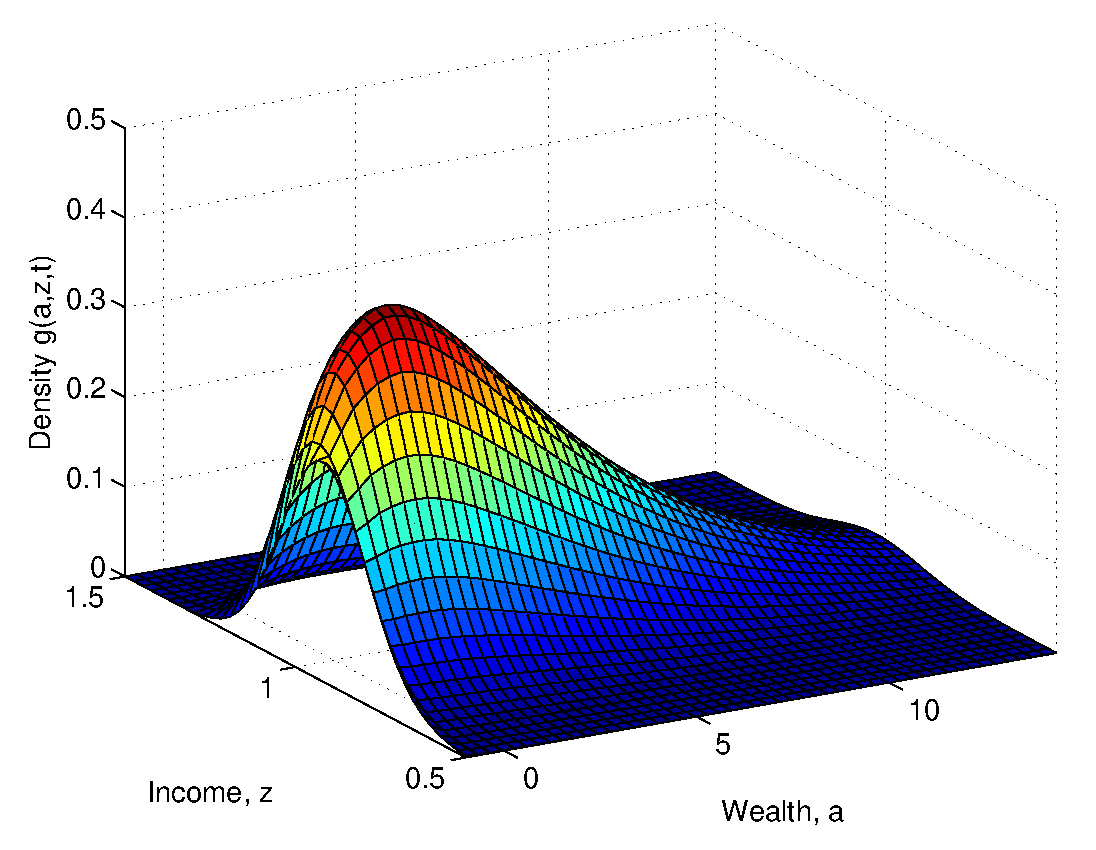
\includegraphics[width=.6\textwidth]{./figures/density_steadystate.eps}
	\end{figure}
\end{frame}


%%%%%%%%%%%%%%%%%%%%%%%%%%  SLIDE   %%%%%%%%%%%%%%%%%%%%%%%%%%%%%%%%
\begin{frame}{What you'll be able to do at end of this course segment}
	\begin{itemize}
		\item Experiment: effect of one-time redistribution of wealth
	\end{itemize}
	\begin{figure}[h]
		\centering
		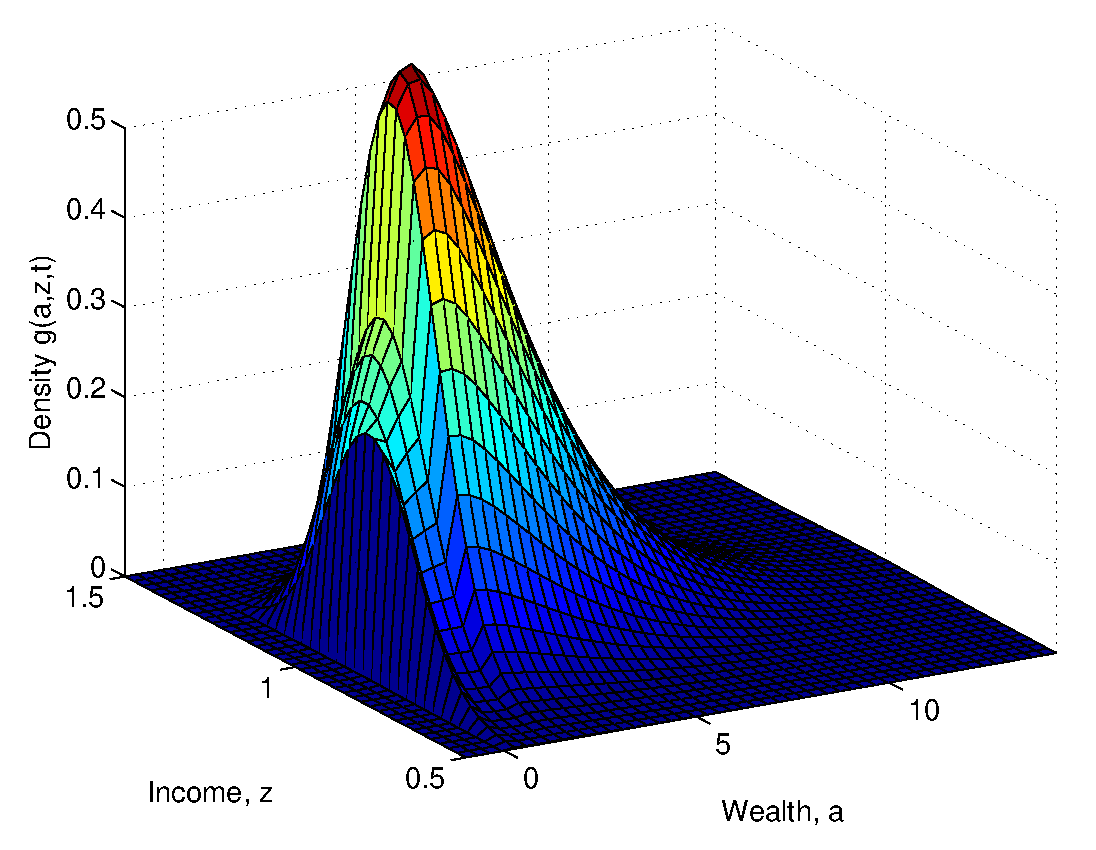
\includegraphics[width=.6\textwidth]{./figures/density_initial.eps}
	\end{figure}
\end{frame}



%%%%%%%%%%%%%%%%%%%%%%%%%%  SLIDE   %%%%%%%%%%%%%%%%%%%%%%%%%%%%%%%%
\begin{frame}{What you'll be able to do at end of this course segment}
	\vspace{2.5cm}
	\begin{center}
		{\large Video of convergence back to steady state}\\ 
		{\scriptsize \url{https://www.dropbox.com/s/op5u2nlifmmer2o/distribution_tax.mp4?dl=0}}
	\end{center}
\end{frame}



%%%%%%%%%%%%%%%%%%%%%%%%%%  SLIDE   %%%%%%%%%%%%%%%%%%%%%%%%%%%%%%%%
\begin{frame}{Outline}
\thispagestyle{empty}
\addtocounter{framenumber}{-1}

Part 1: 30 empirical regularities about inequality
\begin{enumerate}
\item Wage inequality
\item Earnings inequality
\item Individual- versus household-level inequality
\item Government taxes and transfers
\item Consumption and wealth inequality
\end{enumerate}

\end{frame}



%%%%%%%%%%%%%%%%%%%%%%%%%%  SLIDE   %%%%%%%%%%%%%%%%%%%%%%%%%%%%%%%%
\begin{transitionframe}
	{\color{white} \Huge \textbf{Part 1: 30 Facts about Inequality} \vspace{2mm}}
\end{transitionframe}


%%%%%%%%%%%%%%%%%%%%%%%%%%  SLIDE   %%%%%%%%%%%%%%%%%%%%%%%%%%%%%%%%
\begin{frame}{Overview}
\begin{witemize}
\item Document 30 \textbf{empirical regularities} (ER) about inequality

\item Knowing consensus ERs is critical for quantitative and applied theory research:
\begin{enumerate}
	\item Build theories (models) to explain ERs

	\item Models we use to study counter-factuals should be consistent with ERs
\end{enumerate}

\item Main reference: Heathcote-Perri-Violante-Zhang (2023) (\textbf{HPVZ}), also Acemoglu-Autor (2011) (\textbf{AA})

{\footnotesize Also work by: Acemoglu, Autor, Picketty, Saez, ...}

\item Organizing framework: household budget constraint
\begin{equation*}
	c + s = \sum_i^N w_i h_i + d + T^p + T^g - \tau
\end{equation*}

\end{witemize}
\end{frame}


%%%%%%%%%%%%%%%%%%%%%%%%%%  SLIDE   %%%%%%%%%%%%%%%%%%%%%%%%%%%%%%%%
\begin{frame}{}
	\begin{figure}
		\includegraphics[scale=0.35]{./figures/inequality_wage_1}
	\vspace*{-4mm}
	\begin{flushleft}
		{\scriptsize \hspace{6mm} \textbf{Note:} This is Figure 6 in HPVZ. Sample: CPS, working-age individuals with minimum labor force attachment.}
	\end{flushleft}	
	\end{figure}

	\vspace{2mm}
	{\color{blue}\textbf{ER1}}: Wage dispersion has been rising steadily for men and women, but less so since 2000
\end{frame}


%%%%%%%%%%%%%%%%%%%%%%%%%%  SLIDE   %%%%%%%%%%%%%%%%%%%%%%%%%%%%%%%%
\begin{frame}{}
	\begin{figure}
		\includegraphics[scale=0.35]{./figures/inequality_wage_1}
	\vspace*{-4mm}
	\begin{flushleft}
		{\scriptsize \hspace{6mm} \textbf{Note:} This is Figure 6 in HPVZ. Sample: CPS, working-age individuals with minimum labor force attachment.}
	\end{flushleft}	
	\end{figure}

	\vspace{2mm}
	{\color{blue}\textbf{ER2}}: Wage inequality systematically lower for women, only started rising in 1980
\end{frame}


%%%%%%%%%%%%%%%%%%%%%%%%%%  SLIDE   %%%%%%%%%%%%%%%%%%%%%%%%%%%%%%%%
\begin{frame}{}
	\begin{figure}
		\includegraphics[scale=0.4]{./figures/inequality_wage_2}
	\vspace*{-2mm}
	\begin{flushleft}
		{\scriptsize \hspace{6mm} \textbf{Note:} This is Figure 7 in HPVZ. Sample: CPS, working-age individuals with minimum labor force attachment.}
	\end{flushleft}	
	\end{figure}

	\vspace{2mm}
	{\color{blue}\textbf{ER3}}: Rise in wage inequality comes from top of distribution, especially since 1990 
\end{frame}


%%%%%%%%%%%%%%%%%%%%%%%%%%  SLIDE   %%%%%%%%%%%%%%%%%%%%%%%%%%%%%%%%
\begin{frame}{}
	\begin{figure}
		\includegraphics[scale=0.4]{./figures/inequality_wage_2}
	\vspace*{-2mm}
	\begin{flushleft}
		{\scriptsize \hspace{6mm} \textbf{Note:} This is Figure 7 in HPVZ. Sample: CPS, working-age individuals with minimum labor force attachment.}
	\end{flushleft}	
	\end{figure}

	\vspace{2mm}
	{\color{blue}\textbf{ER4}}: Little to no rise in wage dispersion in bottom half of distribution
\end{frame}


%%%%%%%%%%%%%%%%%%%%%%%%%%  SLIDE   %%%%%%%%%%%%%%%%%%%%%%%%%%%%%%%%
\begin{frame}{}
	\begin{figure}
		\includegraphics[scale=0.32]{./figures/inequality_wage_12}
	\vspace*{-2mm}
	\begin{flushleft}
		{\scriptsize \hspace{6mm} \textbf{Note:} This is Figure 7 in AA. Sample: CPS, full-time full-year workers.}
	\end{flushleft}	
	\end{figure}
\end{frame}


%%%%%%%%%%%%%%%%%%%%%%%%%%  SLIDE   %%%%%%%%%%%%%%%%%%%%%%%%%%%%%%%%
\begin{frame}{}
	\begin{figure}
		\includegraphics[scale=0.4]{./figures/inequality_wage_3}
	\vspace*{-2mm}
	\begin{flushleft}
		{\scriptsize \hspace{6mm} \textbf{Note:} This is Figure 7 in HPVZ. Sample: CPS, working-age individuals with minimum labor force attachment.}
	\end{flushleft}	
	\end{figure}

	\vspace{2mm}
	{\color{blue}\textbf{ER3}} and {\color{blue}\textbf{ER4}} same pattern for men and women 
\end{frame}


%%%%%%%%%%%%%%%%%%%%%%%%%%  SLIDE   %%%%%%%%%%%%%%%%%%%%%%%%%%%%%%%%
\begin{frame}{}
	\begin{figure}
		\includegraphics[scale=0.4]{./figures/inequality_wage_4}
	\vspace*{-2mm}
	\begin{flushleft}
		{\scriptsize \hspace{6mm} \textbf{Note:} This is Figure 8 in HPVZ. Sample: CPS, working-age individuals with minimum labor force attachment.}
	\end{flushleft}	
	\end{figure}

	\vspace{2mm}
	{\color{blue}\textbf{ER5}}: Large rise in ratio of average hourly wages with more / less than 16 years of schooling from 1980 until mid-2000s
\end{frame}


%%%%%%%%%%%%%%%%%%%%%%%%%%  SLIDE   %%%%%%%%%%%%%%%%%%%%%%%%%%%%%%%%
\begin{frame}{}
	\begin{figure}
		\includegraphics[scale=0.35]{./figures/inequality_wage_10}
	\vspace*{-2mm}
	\begin{flushleft}
		{\scriptsize \hspace{6mm} \textbf{Note:} This is Figure 1 in AA. Sample: March CPS, log weekly wages for full-time full-year workers.}
	\end{flushleft}	
	\end{figure}
\end{frame}


%%%%%%%%%%%%%%%%%%%%%%%%%%  SLIDE   %%%%%%%%%%%%%%%%%%%%%%%%%%%%%%%%
\begin{frame}{}
	\begin{figure}
		\includegraphics[scale=0.35]{./figures/inequality_wage_11}
	\vspace*{-2mm}
	\begin{flushleft}
		{\scriptsize \hspace{6mm} \textbf{Note:} This is Figure 2 in AA. Sample: March CPS, log weekly wages for full-time full-year workers.}
	\end{flushleft}	
	\end{figure}
\end{frame}


%%%%%%%%%%%%%%%%%%%%%%%%%%  SLIDE   %%%%%%%%%%%%%%%%%%%%%%%%%%%%%%%%
\begin{frame}{}
	\begin{figure}
		\includegraphics[scale=0.4]{./figures/inequality_wage_4}
	\vspace*{-2mm}
	\begin{flushleft}
		{\scriptsize \hspace{6mm} \textbf{Note:} This is Figure 8 in HPVZ. Sample: CPS, working-age individuals with minimum labor force attachment.}
	\end{flushleft}	
	\end{figure}

	\vspace{2mm}
	{\color{blue}\textbf{ER6}}: Ratio in average hourly wage of 45-55 year-olds vs. 25-35 year-olds rises steadily from mid-1970s to mid-1990s
\end{frame}


%%%%%%%%%%%%%%%%%%%%%%%%%%  SLIDE   %%%%%%%%%%%%%%%%%%%%%%%%%%%%%%%%
\begin{frame}{}
	\begin{figure}
		\includegraphics[scale=0.4]{./figures/inequality_wage_5}
	\vspace*{-2mm}
	\begin{flushleft}
		{\scriptsize \hspace{6mm} \textbf{Note:} This is Figure 8 in HPVZ. Sample: CPS, working-age individuals with minimum labor force attachment.}
	\end{flushleft}	
	\end{figure}

	\vspace{2mm}
	{\color{blue}\textbf{ER7}}: Men earned 40-70\% more than women before 1990 but only 20\% more in 2020
\end{frame}


%%%%%%%%%%%%%%%%%%%%%%%%%%  SLIDE   %%%%%%%%%%%%%%%%%%%%%%%%%%%%%%%%
\begin{frame}{}
	\begin{figure}
		\includegraphics[scale=0.4]{./figures/inequality_wage_5}
	\vspace*{-2mm}
	\begin{flushleft}
		{\scriptsize \hspace{6mm} \textbf{Note:} This is Figure 8 in HPVZ. Sample: CPS, working-age individuals with minimum labor force attachment.}
	\end{flushleft}	
	\end{figure}

	\vspace{2mm}
	{\color{blue}\textbf{ER8}}: Ratio of average hourly wages for White and Black workers has fallen slowly  
\end{frame}


%%%%%%%%%%%%%%%%%%%%%%%%%%  SLIDE   %%%%%%%%%%%%%%%%%%%%%%%%%%%%%%%%
\begin{frame}{Summary: wage inequality}

\begin{witemize}
\item Wage dispersion has been rising steadily for men and women, but less so since 2000

\item Wage dispersion at top of distribution (above median) steadily rising since 1960, while relatively stable at bottom of distribution (below median) over last 20 years

\item Gender wage gap continues to narrow, while racial wage gaps are falling slowly

\item Rise of the college premium 1980 to mid-2000s (massive literature)

\item Wage differentials by education, age, and race groups have stabilized since 2000

\end{witemize}
\end{frame}


%%%%%%%%%%%%%%%%%%%%%%%%%%  SLIDE   %%%%%%%%%%%%%%%%%%%%%%%%%%%%%%%%
\begin{frame}{}
	\vspace{4mm}
	\begin{figure}
		\includegraphics[scale=0.32]{./figures/inequality_polarization_1}
	\vspace*{-2mm}
	\begin{flushleft}
		{\scriptsize \hspace{6mm} \textbf{Note:} This is Figure 9 in AA. Sample: May/ORG CPS, all workers excluding military and self-employed.}
	\end{flushleft}	
	\end{figure}

	\vspace{-2mm}
	{\color{blue}\textbf{ER9}}: Wage growth was monotonic (along income distribution) until 1980s but has become U-shaped (``polarized'') since 
\end{frame}


%%%%%%%%%%%%%%%%%%%%%%%%%%  SLIDE   %%%%%%%%%%%%%%%%%%%%%%%%%%%%%%%%
\begin{frame}{}
	\begin{figure}
		\includegraphics[scale=0.4]{./figures/inequality_polarization_3}
	\vspace*{-2mm}
	\begin{flushleft}
		{\scriptsize \hspace{6mm} \textbf{Note:} This is Figure 8 in HPVZ. Sample: CPS, working-age individuals with minimum labor force attachment.}
	\end{flushleft}	
	\end{figure}

	\vspace{2mm}
	{\color{blue}\textbf{ER9}}: Since 1980 wages of abstract cognitive (highest paid) and non-routine manual (lowest-paid) have increased relative to routine occupations (\textbf{wage polarization}) 
\end{frame}


%%%%%%%%%%%%%%%%%%%%%%%%%%  SLIDE   %%%%%%%%%%%%%%%%%%%%%%%%%%%%%%%%
\begin{frame}{}
	\vspace{4mm}
	\begin{figure}
		\includegraphics[scale=0.32]{./figures/inequality_polarization_2}
	\vspace*{-2mm}
	\begin{flushleft}
		{\scriptsize \hspace{6mm} \textbf{Note:} This is Figure 10 in AA. Sample: Census IMPUS and Census ACS.}  
	\end{flushleft}	
	\end{figure}

	\vspace{0mm}
	{\color{blue}\textbf{ER10}}: Simultaneous growth of employment in high-skill/wage and low-skill/wage occupations (\textbf{job polarization}) 
\end{frame}


%%%%%%%%%%%%%%%%%%%%%%%%%%  SLIDE   %%%%%%%%%%%%%%%%%%%%%%%%%%%%%%%%
\begin{frame}{Summary: wage and job polarization}

\begin{witemize}
\item Wage growth was monotonic along income distribution until 1980s but has become polarized since then

\item At the same time, employment shares have risen the most for low- and high-wage occupations $\to$ hollowing out of employment distribution 

\item Readings:
\begin{itemize}
	\item Autor-Levy-Murnane (2003): routinization hypothesis
	\item Acemoglu-Autor (2011) Handbook chapter 
	\item Autor-Dorn (2013): rise of low-skill service jobs
\end{itemize}
\end{witemize}
\end{frame}


%%%%%%%%%%%%%%%%%%%%%%%%%%  SLIDE   %%%%%%%%%%%%%%%%%%%%%%%%%%%%%%%%
\begin{frame}{}
	\vspace{4mm}
	\begin{figure}
		\includegraphics[scale=0.28]{./figures/inequality_earnings_1}
	\end{figure}

	\vspace{0mm}
	{\color{blue}\textbf{ER11}}: Income share of top 10\% was high before WW2, fell and remained low until 1980, rising strongly since 
\end{frame}


%%%%%%%%%%%%%%%%%%%%%%%%%%  SLIDE   %%%%%%%%%%%%%%%%%%%%%%%%%%%%%%%%
\begin{frame}{}
	\vspace{4mm}
	\begin{figure}
		\includegraphics[scale=0.28]{./figures/inequality_earnings_2}
	\end{figure}

	\vspace{0mm}
	{\color{blue}\textbf{ER12}}: Rise in income share since 1980 driven almost entirely by top 1\%
\end{frame}


%%%%%%%%%%%%%%%%%%%%%%%%%%  SLIDE   %%%%%%%%%%%%%%%%%%%%%%%%%%%%%%%%
\begin{frame}{}
	\begin{figure}
		\includegraphics[scale=0.4]{./figures/inequality_earnings_3}
	\vspace*{-2mm}
	\begin{flushleft}
		{\scriptsize \hspace{6mm} \textbf{Note:} This is Figure 10 in HPVZ. Sample: CPS, working-age individuals with minimum labor force attachment.}
	\end{flushleft}	
	\end{figure}

	\vspace{0mm}
	{\color{blue}\textbf{ER13}}: Correlation between hours and wages rose until 1980s, positive and stable since 
\end{frame}


%%%%%%%%%%%%%%%%%%%%%%%%%%  SLIDE   %%%%%%%%%%%%%%%%%%%%%%%%%%%%%%%%
\begin{frame}{}
	\begin{figure}
		\includegraphics[scale=0.4]{./figures/inequality_earnings_4}
	\vspace*{-2mm}
	\begin{flushleft}
		{\scriptsize \hspace{6mm} \textbf{Note:} This is Figure 11 in HPVZ. Sample: CPS, workers including those with little to no hours.}
	\end{flushleft}	
	\end{figure}

	\vspace{0mm}
	{\color{blue}\textbf{ER14}}: Stark increase in earnings inequality at the top driven by rising wage gap at the top. Top wages doubled last 50 years, middle wages flat. (Weeks worked flat.)
\end{frame}


%%%%%%%%%%%%%%%%%%%%%%%%%%  SLIDE   %%%%%%%%%%%%%%%%%%%%%%%%%%%%%%%%
\begin{frame}{}
	\begin{figure}
		\includegraphics[scale=0.4]{./figures/inequality_earnings_5}
	\vspace*{-2mm}
	\begin{flushleft}
		{\scriptsize \hspace{6mm} \textbf{Note:} This is Figure 11 in HPVZ. Sample: CPS, workers including those with little to no hours.}
	\end{flushleft}	
	\end{figure}

	\vspace{-2mm}
	{\color{blue}\textbf{ER15}}: Earnings inequality at the bottom rises throughout sample period, driven by decline in weeks worked by low-earners 
\end{frame}


%%%%%%%%%%%%%%%%%%%%%%%%%%  SLIDE   %%%%%%%%%%%%%%%%%%%%%%%%%%%%%%%%
\begin{frame}{}
	\begin{figure}
		\includegraphics[scale=0.4]{./figures/inequality_earnings_5}
	\vspace*{-2mm}
	\begin{flushleft}
		{\scriptsize \hspace{6mm} \textbf{Note:} This is Figure 11 in HPVZ. Sample: CPS, workers including those with little to no hours.}
	\end{flushleft}	
	\end{figure}

	\vspace{0mm}
	{\color{blue}\textbf{ER16}}: Weeks worked by low-earners very cyclical
\end{frame}


%%%%%%%%%%%%%%%%%%%%%%%%%%  SLIDE   %%%%%%%%%%%%%%%%%%%%%%%%%%%%%%%%
\begin{frame}{}
	\begin{figure}
		\includegraphics[scale=0.4]{./figures/inequality_earnings_7}
	\end{figure}

	\vspace{2mm}
	{\color{blue}\textbf{ER17}}: labor share (in aggregate income) has fallen since 1980
\end{frame}


%%%%%%%%%%%%%%%%%%%%%%%%%%  SLIDE   %%%%%%%%%%%%%%%%%%%%%%%%%%%%%%%%
\begin{frame}{Summary: earnings inequality}

\begin{witemize}
\item Earnings dispersion at the top driven by long-run trends, while at the bottom strongly cyclical

\item Earnings dispersion at the top is about changes in wages (hours stable)

\item Earnings dispersion at the bottom is about hours (annual weeks worked)

\item Labor share has fallen since 1980 (massive literature!)
\end{witemize}
\end{frame}


%%%%%%%%%%%%%%%%%%%%%%%%%%  SLIDE   %%%%%%%%%%%%%%%%%%%%%%%%%%%%%%%%
\begin{frame}{}
	\begin{figure}
		\includegraphics[scale=0.35]{./figures/inequality_household_1}
	\vspace*{-4mm}
	\begin{flushleft}
		{\scriptsize \hspace{6mm} \textbf{Note:} This is Figure 12 in HPVZ. Sample: CPS, all households with one member aged 25-60.}
	\end{flushleft}	
	\end{figure}

	\vspace{0mm}
	{\color{blue}\textbf{ER18}}: Rising dispersion in household earnings at the top (slight attenuation compared to individual earnings)
\end{frame}


%%%%%%%%%%%%%%%%%%%%%%%%%%  SLIDE   %%%%%%%%%%%%%%%%%%%%%%%%%%%%%%%%
\begin{frame}{}
	\begin{figure}
		\includegraphics[scale=0.35]{./figures/inequality_household_1}
	\vspace*{-4mm}
	\begin{flushleft}
		{\scriptsize \hspace{6mm} \textbf{Note:} This is Figure 12 in HPVZ. Sample: CPS, all households with one member aged 25-60.}
	\end{flushleft}	
	\end{figure}

	\vspace{0mm}
	{\color{blue}\textbf{ER19}}: Large spikes in male earnings dispersion during recent recessions strongly attenuated in household earnings dispersion
\end{frame}


%%%%%%%%%%%%%%%%%%%%%%%%%%  SLIDE   %%%%%%%%%%%%%%%%%%%%%%%%%%%%%%%%
\begin{frame}{}
	\begin{figure}
		\includegraphics[scale=0.4]{./figures/inequality_household_2}
	\vspace*{-2mm}
	\begin{flushleft}
		{\scriptsize \hspace{6mm} \textbf{Note:} This is Figure 13 in HPVZ. Sample: CPS, all households with one member aged 25-60.}
	\end{flushleft}	
	\end{figure}

	\vspace{0mm}
	{\color{blue}\textbf{ER20}}: Large decline in household income pooling. In 1970, income pooling reduced variance of individual earnings dispersion by 60\%, down to 35\% today
\end{frame}


%%%%%%%%%%%%%%%%%%%%%%%%%%  SLIDE   %%%%%%%%%%%%%%%%%%%%%%%%%%%%%%%%
\begin{frame}{}
	\begin{figure}
		\includegraphics[scale=0.35]{./figures/inequality_household_3}
	\vspace*{-2mm}
	\begin{flushleft}
		{\scriptsize \hspace{6mm} \textbf{Note:} This is Figure 13 in HPVZ. Sample: CPS, all households with one member aged 25-60.}
	\end{flushleft}	
	\end{figure}

	\vspace{0mm}
	{\color{blue}\textbf{ER21}}: Decline in gender gap and increased sorting main drivers of lower household pooling
\end{frame}


%%%%%%%%%%%%%%%%%%%%%%%%%%  SLIDE   %%%%%%%%%%%%%%%%%%%%%%%%%%%%%%%%
\begin{frame}{Summary: individual- vs. household-level earnings inequality}

\begin{witemize}
\item Household is potentially important source of insurance and redistribution due to income pooling

\item Correlation between earnings within couples has increased (sorting)

\item Gender gap in earnings has declined 

\item Consequently: within-household insurance and redistribution less important
\end{witemize}
\end{frame}


%%%%%%%%%%%%%%%%%%%%%%%%%%  SLIDE   %%%%%%%%%%%%%%%%%%%%%%%%%%%%%%%%
\begin{frame}{}
	\begin{figure}
		\includegraphics[scale=0.3]{./figures/inequality_government_1}
	\vspace*{-2mm}
	\begin{flushleft}
		{\scriptsize \hspace{6mm} \textbf{Note:} This is Figure 16 in HPVZ. Sample: CPS, all households with one member aged 25-60.}
	\end{flushleft}	
	\end{figure}

	\vspace{0mm}
	{\color{blue}\textbf{ER22}}: Trend growth in market income at top and middle. No trend growth at bottom but large cyclicality
\end{frame}


%%%%%%%%%%%%%%%%%%%%%%%%%%  SLIDE   %%%%%%%%%%%%%%%%%%%%%%%%%%%%%%%%
\begin{frame}{}
	\begin{figure}
		\includegraphics[scale=0.3]{./figures/inequality_government_1}
	\vspace*{-2mm}
	\begin{flushleft}
		{\scriptsize \hspace{6mm} \textbf{Note:} This is Figure 16 in HPVZ. Sample: CPS, all households with one member aged 25-60.}
	\end{flushleft}	
	\end{figure}

	\vspace{0mm}
	{\color{blue}\textbf{ER23}}: Transfers large and rising at bottom, mute cyclicality in disposable income
\end{frame}


%%%%%%%%%%%%%%%%%%%%%%%%%%  SLIDE   %%%%%%%%%%%%%%%%%%%%%%%%%%%%%%%%
\begin{frame}{}
	\begin{figure}
		\includegraphics[scale=0.3]{./figures/inequality_government_1}
	\vspace*{-2mm}
	\begin{flushleft}
		{\scriptsize \hspace{6mm} \textbf{Note:} This is Figure 16 in HPVZ. Sample: CPS, all households with one member aged 25-60.}
	\end{flushleft}	
	\end{figure}

	\vspace{0mm}
	{\color{blue}\textbf{ER24}}: Taxes mute rise in disposable income dispersion at the top
\end{frame}


%%%%%%%%%%%%%%%%%%%%%%%%%%  SLIDE   %%%%%%%%%%%%%%%%%%%%%%%%%%%%%%%%
\begin{frame}{}
	\begin{figure}
		\includegraphics[scale=0.38]{./figures/inequality_government_2}
	\vspace*{-2mm}
	\begin{flushleft}
		{\scriptsize \hspace{6mm} \textbf{Note:} This is Figure 17 in HPVZ. Sample: CPS, all households with one member aged 25-60.}
	\end{flushleft}	
	\end{figure}
\end{frame}


%%%%%%%%%%%%%%%%%%%%%%%%%%  SLIDE   %%%%%%%%%%%%%%%%%%%%%%%%%%%%%%%%
\begin{frame}{}
	\begin{figure}
		\includegraphics[scale=0.3]{./figures/inequality_government_3}
	\vspace*{-2mm}
	\begin{flushleft}
		{\scriptsize \hspace{6mm} \textbf{Note:} This is Figure 18 in HPVZ. Sample: CPS, all households with one member aged 25-60.}
	\end{flushleft}	
	\end{figure}
\end{frame}


%%%%%%%%%%%%%%%%%%%%%%%%%%  SLIDE   %%%%%%%%%%%%%%%%%%%%%%%%%%%%%%%%
\begin{frame}{}
	\begin{figure}
		\includegraphics[scale=0.38]{./figures/inequality_government_4}
	\end{figure}
\end{frame}


%%%%%%%%%%%%%%%%%%%%%%%%%%  SLIDE   %%%%%%%%%%%%%%%%%%%%%%%%%%%%%%%%
\begin{frame}{Summary: insurance and redistribution}
\begin{witemize}
\item Large rise in market income dispersion 

\item Income pooling reduces dispersion in household income dispersion, but increasingly less so

\item At bottom (below median), inequality in market (pretax) income strongly counter-cyclical (unemployment)

\item Transfers (and taxes to lesser extent) compress inequality and dampen cyclicality

\item Transfers and automatic stabilizers during Covid so large that disposable income inequality declined for first time across 8 last recessions

\end{witemize}
\end{frame}


%%%%%%%%%%%%%%%%%%%%%%%%%%  SLIDE   %%%%%%%%%%%%%%%%%%%%%%%%%%%%%%%%
\begin{frame}{}
	\begin{figure}
		\includegraphics[scale=0.3]{./figures/inequality_wealth_1}
	\end{figure}

	\vspace{0mm}
	{\color{blue}\textbf{ER25}}: Wealth inequality fell sharply in first half of 20th century, rising steadily since 1970/80 (more in US than in Europe)
\end{frame}


%%%%%%%%%%%%%%%%%%%%%%%%%%  SLIDE   %%%%%%%%%%%%%%%%%%%%%%%%%%%%%%%%
\begin{frame}{}
	\begin{figure}
		\includegraphics[scale=0.35]{./figures/inequality_wealth_2}
	\end{figure}

	\vspace{2mm}
	{\color{blue}\textbf{ER26}}: Wealth distribution is right-skewed and has a fat right tail (Pareto distributed)
\end{frame}


%%%%%%%%%%%%%%%%%%%%%%%%%%  SLIDE   %%%%%%%%%%%%%%%%%%%%%%%%%%%%%%%%
\begin{frame}{}
	\begin{figure}
		\includegraphics[scale=0.3]{./figures/inequality_wealth_3}
	\end{figure}

	\vspace{2mm}
	{\color{blue}\textbf{ER27}}: Wealth inequality is larger than earnings inequality
\end{frame}


%%%%%%%%%%%%%%%%%%%%%%%%%%  SLIDE   %%%%%%%%%%%%%%%%%%%%%%%%%%%%%%%%
\begin{frame}{}
	\begin{figure}
		\includegraphics[scale=0.4]{./figures/inequality_consumption_2}
	\vspace*{-2mm}
	\begin{flushleft}
		{\scriptsize \hspace{6mm} \textbf{Note:} This is Figure 24 in HPVZ. Sample: PSID, all households with one member aged 25-60.}
	\end{flushleft}	
	\end{figure}

	\vspace{0mm}
	{\color{blue}\textbf{ER28}}: Wealth ratio below median is similar to income ratio, whereas above median it's much larger and growing 
\end{frame}


%%%%%%%%%%%%%%%%%%%%%%%%%%  SLIDE   %%%%%%%%%%%%%%%%%%%%%%%%%%%%%%%%
\begin{frame}{}
	\begin{figure}
		\includegraphics[scale=0.4]{./figures/inequality_consumption_0}
	\vspace*{-2mm}
	\begin{flushleft}
		{\scriptsize \hspace{6mm} \textbf{Note:} This is Figure 22 in HPVZ. Sample: CES and PSID, all households with one member aged 25-60.}
	\end{flushleft}	
	\end{figure}

	\vspace{0mm}
	{\color{blue}\textbf{ER29}}: Consumption inequality is flat over time at top and bottom!!
\end{frame}


%%%%%%%%%%%%%%%%%%%%%%%%%%  SLIDE   %%%%%%%%%%%%%%%%%%%%%%%%%%%%%%%%
\begin{frame}{}
	\begin{figure}
		\includegraphics[scale=0.4]{./figures/inequality_consumption_3}
	\end{figure}
\end{frame}


%%%%%%%%%%%%%%%%%%%%%%%%%%  SLIDE   %%%%%%%%%%%%%%%%%%%%%%%%%%%%%%%%
\begin{frame}{}
	\begin{figure}
		\includegraphics[scale=0.4]{./figures/inequality_consumption_1}
	\vspace*{-2mm}
	\begin{flushleft}
		{\scriptsize \hspace{6mm} \textbf{Note:} This is Figure 16 in HPVZ. Sample: CPS, all households with one member aged 25-60.}
	\end{flushleft}	
	\end{figure}

	\vspace{0mm}
	{\color{blue}\textbf{ER30}}: Consumption differentials small compared to income differentials (at bottom and top)
\end{frame}


%%%%%%%%%%%%%%%%%%%%%%%%%%  SLIDE   %%%%%%%%%%%%%%%%%%%%%%%%%%%%%%%%
\begin{frame}{Summary: wealth and consumption inequality}
\begin{witemize}
\item Wealth inequality fell in first half of 20th century but is rising since 1980

\item Wealth inequality > income inequality > consumption inequality

\item Despite rising income and wealth inequality, consumption inequality has been relatively flat across entire distribution! 

\end{witemize}
\end{frame}


\end{document}

%%%%%%%%%%%%%%%%%%%%%%%%%%  SLIDE   %%%%%%%%%%%%%%%%%%%%%%%%%%%%%%%%
\begin{transitionframe}
	{\color{white} \Huge \textbf{Part 2: Huggett (1993)} \vspace{2mm}}
\end{transitionframe}


%%%%%%%%%%%%%%%%%%%%%%%%%%  SLIDE   %%%%%%%%%%%%%%%%%%%%%%%%%%%%%%%%
\begin{frame}{Model overview}
\begin{witemize}
\item Time is continuous, $t \in [0, \infty)$

\item No aggregate uncertainty $\implies$ focus on one-time, unanticipated (``MIT'') shocks (perfect foresight wrt. macroeconomic aggregates)

\item Continuum of households of measure 1

\item Households face ``uninsurable idiosyncratic income risk''

\item There is a single riskfree asset in zero net supply (= government bond)

\end{witemize}

\vspace{4mm} 
\textbf{Plan:}
\begin{enumerate}
\item Present model in sequence form focusing exposition on individual $i$
\item Recursive representation of competitive equilibrium
\end{enumerate}
\end{frame}


%%%%%%%%%%%%%%%%%%%%%%%%%%  SLIDE   %%%%%%%%%%%%%%%%%%%%%%%%%%%%%%%%
\begin{frame}{Households}

\textbf{Preferences.} The individual lifetime utility of a household $i \in [0, 1]$ is 
\begin{equation*}
	V_{i, 0} = \max_{ \{c_{i, t}\}_{t \geq 0} } \; \mathbb E_0 \int_0^\infty e^{- \rho t} u(c_{i, t}) dt
\end{equation*}


\vspace{5mm}
\textbf{Budget} and \textbf{borrowing constraints}:
\begin{align*}
	\dot a_{i, t} &= y_{i, t} + r_t a_{i, t} - c_{i, t} \\[2pt]
	a_{i, t} &\geq \underline a
\end{align*}


\vspace{5mm}
\textbf{Idiosyncratic income risk}: each $y_{i, t}$ follows a Markov chain
\begin{equation*}
	y_{i, t} \in \{y_1, y_2\} \; \text{ Poisson with intensities } \lambda_1, \lambda_2
\end{equation*}

Later: carries over to $y_{i, t}$ = more general processes, e.g. diffusion 

\end{frame}


%%%%%%%%%%%%%%%%%%%%%%%%%%  SLIDE   %%%%%%%%%%%%%%%%%%%%%%%%%%%%%%%%
\begin{frame}{}

\textbf{Definition.} The problem of household $i$ (in sequence form) is 
	\begin{equation*}\label{HH}\begin{split}
		\max_{\{c_{i, t}\}_{t \geq 0}} \ 
			& \mathbb E_0 \int_0^\infty e^{-\rho t} u(c_{i, t}) dt \quad \quad \mbox{s.t.} \\
			&\dot a_{i, t} = y_{i, t} + r_t a_{i, t} - c_{i, t} \\
			&y_{i, t} \in \{y_1, y_2\} \ \mbox{Poisson with intensities} \ \lambda_1,\lambda_2\\
			&a_{i, t} \geq \ushort a \end{split}
	\end{equation*}
\end{frame}


%%%%%%%%%%%%%%%%%%%%%%%%%%  SLIDE   %%%%%%%%%%%%%%%%%%%%%%%%%%%%%%%%
\begin{frame}{Typical Consumption and Saving Policy Functions}
	\vspace{1cm}
	\includegraphics[width=.45\textwidth]{./figures/HACT_consumption}\qquad
	\includegraphics[width=.45\textwidth]{./figures/HACT_savings}
\end{frame}


%%%%%%%%%%%%%%%%%%%%%%%%%%  SLIDE   %%%%%%%%%%%%%%%%%%%%%%%%%%%%%%%%
\begin{frame}{Typical Stationary Distribution}
	\vspace{1cm}
	\centering
	\includegraphics[width=.5\textwidth]{./figures/HACT_distribution}
\end{frame}





%%%%%%%%%%%%%%%%%%%%%%%%%%  SLIDE   %%%%%%%%%%%%%%%%%%%%%%%%%%%%%%%%
\begin{frame}{Equations for Stationary Equilibrium}\label{equilibrium}
	\vspace{-3mm}
	\begin{align}
		\uncover<1->{\tag{HJB} \rho v_j(a) &= \max_c \ u(c) + v_j'(a)(y_j + r a - c) + \lambda_j(v_{-j}(a) - v_j(a))\\[2ex]}
		\uncover<2->{\tag{KF} 0 &= - \frac{d}{da}[s_j(a)g_j(a)] - \lambda_j g_j(a) + \lambda_{-j} g_{-j}(a),\\[1ex]
			\notag &s_j(a) = y_j + r a - c_j(a) = \mbox{saving policy function from (HJB)},\\[1ex]
			\notag &\int_{\ushort{a}}^\infty (g_1(a) + g_2(a))da = 1, \quad g_1,g_2 \geq 0 \\[2ex]}
		\uncover<3->{\notag S(r) &:= \int_{\ushort{a}}^\infty a g_1(a)da + \int_{\ushort{a}}^\infty a g_2(a)da = B, \qquad B \geq 0 \qquad \qquad \ \mbox{(EQ)}}
	\end{align}
	\begin{itemize}
		\uncover<4->{\item The two PDEs (HJB) and (KF) together with (EQ) fully characterize stationary equilibrium \hyperlink{KFEder}{\beamergotobutton{Derivation of (HJB)}} \hyperlink{KFEder}{\beamergotobutton{(KF)}}}
	\end{itemize}
\end{frame}





%%%%%%%%%%%%%%%%%%%%%%%%%%  SLIDE   %%%%%%%%%%%%%%%%%%%%%%%%%%%%%%%%
\begin{frame}{Transition Dynamics}
	\bi
	\item Needed whenever initial condition $\neq$ stationary distribution
	\bigskip
	\item Equilibrium still coupled systems of HJB and KF equations...
	\bigskip
	\item ... but now \tr{time-dependent}: $v_j(a,\tr{t})$ and $g_j(a,\tr{t})$
	\bigskip
	\item See next slides for equations
	\bigskip
	\item Difficulty: the two PDEs run in opposite directions in time
	\bi
	\medskip
	\item HJB looks forward, runs backwards from terminal condition
	\medskip
	\item KF looks backward, runs forward from initial condition
	\ei
	\ei
\end{frame}


%%%%%%%%%%%%%%%%%%%%%%%%%%  SLIDE   %%%%%%%%%%%%%%%%%%%%%%%%%%%%%%%%
\begin{frame}{Transition Dynamics}
	\vspace{-5mm}
	{\small 
		\begin{align}
			\tag{EQ} B = & \int_{\ushort{a}}^\infty a g_1(a,t)da + \int_{\ushort{a}}^\infty a g_2(a,t)da\\[2ex]
			\tag{HJB}\begin{split}
				\rho v_j(a,t) =& \max_c \ u(c) + \partial_a v_j(a,t)(y_j + r(t) a - c)\\
				& + \lambda_j(v_{-j}(a,t) - v_j(a,t)) + \partial_t v_j(a,t), 
			\end{split}\\[2ex]
			\tag{KF}\partial_t g_j(a,t) =& - \partial_a[s_j(a,t)g_j(a,t)] - \lambda_j g_j(a,t) + \lambda_{-j} g_{-j}(a,t),\\[1ex]
			\notag s_j(a,t) =& y_j + r(t) a - c_j(a,t), \quad c_j(a,t) = (u')^{-1}(\partial_a v_j(a,t)),\\[1ex]
			\notag & \int_{\ushort{a}}^\infty (g_1(a,t) + g_2(a,t))da = 1, \quad g_1,g_2 \geq 0
	\end{align}}
	\vspace{-4mm}
	\begin{itemize}
		\item Given initial condition $g_{j,0}(a)$, the two PDEs (HJB) and (KF) together with (EQ) fully characterize equilibrium.
		\medskip
		\item Notation: for any function $f$, $\partial_x f$ means $\frac{\partial f}{\partial x}$
	\end{itemize}
\end{frame}



%%%%%%%%%%%%%%%%%%%%%%%%%%  SLIDE   %%%%%%%%%%%%%%%%%%%%%%%%%%%%%%%%
\begin{frame}{Borrowing Constraints?}
	\begin{itemize}
		\uncover<1->{\item Q: where is borrowing constraint $a \geq \ushort{a}$ in (HJB)?
			\item A: ``in'' boundary condition}
		\bigskip
		\uncover<2->{\item \tr{Result:} $v_j$ must satisfy
			\begin{equation}\label{eq:BC}\tag{BC}v_j'(\ushort{a}) \geq u'(y_j + r \ushort{a}), \quad j=1,2\end{equation}
			\item \tr{Derivation:}
			\smallskip
			\begin{itemize}
				\medskip
				\item the FOC still holds at the borrowing constraint
				\begin{equation}\label{eq:FOC}\tag{FOC}u'(c_j(\ushort{a}))= v_j'(\ushort{a})\end{equation}
				\item for borrowing constraint not to be violated, need
				\begin{equation}\label{eq:s}\tag{$\ast$}s_j(\ushort{a}) = y_j + r \ushort{a} - c_j(\ushort{a}) \geq 0\end{equation}
				\item \eqref{eq:FOC} and \eqref{eq:s} $\Rightarrow$ \eqref{eq:BC}.
		\end{itemize}}
		%\bigskip
		%\uncover<3->{\item See slides on viscosity solutions for more rigorous discussion \\
		%	{\scriptsize \url{http://www.princeton.edu/~moll/viscosity_slides.pdf}}}
	\end{itemize}
\end{frame}



%%%%%%%%%%%%%%%%%%%%%%%%%%  SLIDE   %%%%%%%%%%%%%%%%%%%%%%%%%%%%%%%%
\begin{frame}{Plan}
	\begin{itemize}
		\item  \tr{New theoretical results:}
		\be
		\medskip
		\item analytics: consumption, saving, MPCs of the poor
		\bigskip
		\item closed-form for wealth distribution with 2 income types
		\bigskip
		\item unique stationary equilibrium if IES $\geq 1$ (sufficient condition)
		\bigskip
		\item ``soft" borrowing constraints
		\ee
		\medskip
		Note: for 1., 2. and 4. analyze \tr{partial equilibrium} with $r<\rho$
		\bigskip
		\medskip
		\item \tr{Computational algorithm:}
		\bi
		\bigskip
		\item problems with non-convexities
		\bigskip
		\item transition dynamics
		\ei
	\end{itemize}
\end{frame}





%\begin{frame}{Result 1: Consumption, Saving Behavior of the Poor}
%\vspace{-3mm}
%Consumption/saving behavior near borrowing constraint depends on:
%\begin{enumerate}
%\medskip
%\item tightness of constraint
%\medskip
%\item properties of $u$ as $c\rightarrow 0$
%\end{enumerate}
%\pause
%\bigskip
%\tr{Assumption 1:}\newline \emph{As $a \rightarrow \ushort{a}$, coefficient of absolute risk aversion $R(c) := -u''(c)/u'(c)$ remains finite}
%$$ - \frac{u''(y_1 +  r\ushort{a})}{u'(y_1 + r\ushort{a})}<\infty$$
%\vspace{-3mm}
%\bi 
%\item will show: A1 $\Rightarrow$ borrowing constraint ``matters" (in fact, it's an $\Leftrightarrow$)
%\medskip
%\ei
%\pause
%How to read A1?
%\bi
%\medskip
%\item for ``standard" $u$ functions (e.g. CRRA): equivalent to $\ushort{a}>-y_1/r$
%\medskip
%\item but weaker: \tr{only violated if both} $\ushort{a}=-y_1/r$ \tr{and} $-\tfrac{u''(0)}{u'(0)}=\infty$
%%IN THIS CASE BORROWING CONSTRAINT IS UNINTERESTING, IN ALL OTHER CASES IT WILL BE
%\medskip
%\item e.g. if $u'(c)= e^{-\theta c}$: A1 holds \& constraint matters even if $\ushort{a}=-\tfrac{y_1}{r}$
%\ei
%\end{frame}



%%%%%%%%%%%%%%%%%%%%%%%%%%  SLIDE   %%%%%%%%%%%%%%%%%%%%%%%%%%%%%%%%
\begin{transitionframe}
	{\color{white} \Huge \textbf{Theoretical Results} \vspace{2mm}}
\end{transitionframe}


%%%%%%%%%%%%%%%%%%%%%%%%%%  SLIDE   %%%%%%%%%%%%%%%%%%%%%%%%%%%%%%%%
\begin{frame}{Result 1: Consumption, Saving Behavior of the Poor}
	Consumption/saving behavior near borrowing constraint depends on:
	\begin{enumerate}
		\item tightness of constraint
		\item properties of $u$ as $c\rightarrow 0$
	\end{enumerate}
	\pause
	\medskip
	\tr{Assumption 1:}\newline \emph{As $a \rightarrow \ushort{a}$, coefficient of absolute risk aversion $R(c) := -u''(c)/u'(c)$ remains finite}
	$$ - \frac{u''(y_1 +  r\ushort{a})}{u'(y_1 + r\ushort{a})}<\infty$$
	\vspace{-3mm}
	\bi 
	\item will show: A1 $\Rightarrow$ borrowing constraint ``matters" (in fact, it's an $\Leftrightarrow$)
	\medskip
	\ei
	\pause
	How to read A1?
	\bi
	\item ``standard" utility functions, e.g. CRRA, satisfy $-\tfrac{u''(0)}{u'(0)}=\infty$
	\item hence for standard utility functions A1 equivalent to $\ushort{a}>-y_1/r$, i.e. constraint matters if it is tighter than ``natural borrowing constraint"
	\item  but weaker: e.g. if $u'(c)= e^{-\theta c}$, constraint matters even if $\ushort{a}=-\tfrac{y_1}{r}$
	%\item for ``standard" $u$ functions (e.g. CRRA): equivalent to $\ushort{a}>-y_1/r$
	%\medskip
	%\item but weaker: \tr{only violated if both} $\ushort{a}=-y_1/r$ \tr{and} $-\tfrac{u''(0)}{u'(0)}=\infty$
	%%IN THIS CASE BORROWING CONSTRAINT IS UNINTERESTING, IN ALL OTHER CASES IT WILL BE
	%\medskip
	%\item e.g. if $u'(c)= e^{-\theta c}$: A1 holds \& constraint matters even if $\ushort{a}=-\tfrac{y_1}{r}$
	\ei
\end{frame}



%%%%%%%%%%%%%%%%%%%%%%%%%%  SLIDE   %%%%%%%%%%%%%%%%%%%%%%%%%%%%%%%%
\begin{frame}{Result 1: Consumption, Saving Behavior of the Poor}
	Rough version of Proposition: under A1 policy functions look like this\\
	\vspace{1cm}
	\includegraphics[width=.45\textwidth]{./figures/HACT_consumption}\qquad
	\includegraphics[width=.45\textwidth]{./figures/HACT_savings}
\end{frame}


%%%%%%%%%%%%%%%%%%%%%%%%%%  SLIDE   %%%%%%%%%%%%%%%%%%%%%%%%%%%%%%%%
\begin{frame}{Result 1: Consumption, Saving Behavior of the Poor}\label{prop:sav}
	\tr{\textbf{Proposition:}} Assume $r<\rho, y_1<y_2$ and that A1 holds.\\ Then saving and consumption policy functions close to $a=\ushort{a}$ satisfy
	\begin{align*}
		s_1(a) &\sim -  \sqrt{2\nu_1}\tr{\sqrt{a - \ushort{a}}}\\[1.2ex]
		c_1(a) &\sim y_1 + r a + \sqrt{2\nu_1}\tr{\sqrt{a - \ushort{a}}}\\[1.2ex]
		c_1'(a) &\sim r + \frac{1}{2} \sqrt{\frac{\nu_1}{2\tr{(a - \ushort{a})}}}
	\end{align*}
	where $\nu_1=$ constant that depends on $r,\rho,\lambda_1,\lambda_2$ etc -- see next slide
	\\
	\bigskip
	{\footnotesize Note: ``$f(a)\sim g(a)$" means $\lim_{a \rightarrow \ushort{a}}f(a)/g(a)=1$, ``$f$ behaves like $g$ close to $\ushort{a}$"}
\end{frame}



%%%%%%%%%%%%%%%%%%%%%%%%%%  SLIDE   %%%%%%%%%%%%%%%%%%%%%%%%%%%%%%%%
\begin{frame}{Result 1: Consumption, Saving Behavior of the Poor}
	\tr{\textbf{Corollary:}} The wealth of worker who keeps $y_1$ converges to borrowing constraint {\tr{in finite time}} at speed governed by $\tr{\nu_1}$:
	%\begin{align*}
	%a(t) - \ushort{a} &\sim \frac{\tr{\nu_1}}{2}\left(\tb{T}-t\right)^2 , \quad 0 \leq t\leq \tb{T}, \quad \mbox{where}\\
	%\tb{T} & := \tb{\mbox{``hitting time"}} = \tb{\sqrt{\tfrac{2(a_0 - \ushort{a})}{\nu_1}}}
	%\end{align*}
	\begin{align*}
		a(t) - \ushort{a} &\sim \frac{\tr{\nu_1}}{2}\left(\tb{T}-t\right)^2, \quad \tb{T} := \tb{\mbox{``hitting time"}} = \tb{\sqrt{\tfrac{2(a_0 - \ushort{a})}{\nu_1}}}, \quad 0 \leq t\leq \tb{T}
	\end{align*}
	Proof: integrate $\dot{a}(t) = - \sqrt{2\tr{\nu_1}}\sqrt{a(t) - \ushort{a}}$\\
	\bigskip
	\pause
	And have analytic solution for speed
	\begin{align*}
		{\tr{\nu_1}} &= \frac{(\rho - r)u'(\ushort{c}_{1}) + \lambda_1 (u'(\ushort{c}_{1}) - u'(\ushort{c}_{2}))}{-u''(\ushort{c}_{1})} \\
		&\approx \tr{(\rho-r)\textrm{IES}(\ushort{c}_1)\ushort{c}_1 + \lambda_1(\ushort{c}_2 - \ushort{c}_1)}
	\end{align*}
\end{frame}




%%%%%%%%%%%%%%%%%%%%%%%%%%  SLIDE   %%%%%%%%%%%%%%%%%%%%%%%%%%%%%%%%
\begin{frame}{Intuition for Result 1: Two Special Cases}
	\bi
	\item What's the role of A1? And why the square root?
	\bigskip
	\item Explain using two special cases with \tr{analytic solution}
	\bigskip
	\item Both cases: \tr{no income uncertainty}
	\ei
\end{frame}


%%%%%%%%%%%%%%%%%%%%%%%%%%  SLIDE   %%%%%%%%%%%%%%%%%%%%%%%%%%%%%%%%
\begin{frame}{Intuition for Result 1: Two Special Cases}
	\bi
	\item Special case 1: A1 holds, \tr{hit} constraint
	\ei
	\centering
	\includegraphics[width=.6\textwidth]{./figures/HACT_example1}
	\bi
	\item Special case 2: A1 violated, \tr{approach} constraint \tr{asymptotically}
	\medskip
	\ei
	\includegraphics[width=.6\textwidth]{./figures/HACT_example2}
\end{frame}


%%%%%%%%%%%%%%%%%%%%%%%%%%  SLIDE   %%%%%%%%%%%%%%%%%%%%%%%%%%%%%%%%
\begin{frame}{}
	\vspace{4mm}
	Special case 1: \tr{hit} constraint
	\bi
	\smallskip
	\item exponential utility $u'(c) = e^{-\theta c}$, tight constraint
	$$\dot{c} = \frac{1}{\theta}(r-\rho), \qquad \dot{a} = y + ra - c, \qquad a \geq 0$$
	\item satisfies A1: $-\frac{u''(y)}{u'(y)} = \theta <\infty$. \uncover<2->{Solution:
		\begin{align*}
			c(t) &= y + \tr{\nu}(\tb{T}-t), \quad a(t) = \frac{\tr{\nu}}{2}(\tb{T}-t)^2, \quad \tr{\nu := \tfrac{\rho-r}{\theta}}
			%\\
			%&\Rightarrow \quad c(a) = y + \sqrt{2 \nu a}
		\end{align*}
	}
	%\item<2->{Solution:}
	\ei
	\vspace{-3mm}
	Special case 2: only \tr{approach} constraint \tr{asymptotically}
	\bi
	\medskip
	\item CRRA utility $u'(c) = c^{-\gamma}$, loose constraint 
	$$\frac{\dot{c}}{c} = \frac{1}{\gamma}(r-\rho), \qquad \dot{a} = y +  ra - c, \qquad a \geq \tr{\ushort{a} =-\frac{y}{r}}$$
	\item violates A1: $-\frac{u''(y +  ra)}{u'(y + ra)} \rightarrow \infty$ as $a\rightarrow \ushort{a}$. \uncover<3->{Solution:
		$$c(t) = y + (r + \tr{\eta})a(t), \quad a(t) - \ushort{a} = (a_0 - \ushort{a}) e^{-\tr{\eta} t}, \quad \tr{\eta:=\tfrac{\rho-r}{\gamma}}  $$ }
	\ei
\end{frame}


%%%%%%%%%%%%%%%%%%%%%%%%%%  SLIDE   %%%%%%%%%%%%%%%%%%%%%%%%%%%%%%%%
\begin{frame}{Intuition for Result 1: Two Special Cases}
	\bi
	\item Special case 1: A1 holds, \tr{hit} constraint
	\ei
	\centering
	\includegraphics[width=.6\textwidth]{./figures/HACT_example1}
	\bi
	\item Special case 2: A1 violated, \tr{approach} constraint \tr{asymptotically}
	\medskip
	\ei
	\includegraphics[width=.6\textwidth]{./figures/HACT_example2}
\end{frame}

%\begin{frame}{Special Case 1: \tr{Exponential utility} $u'(c)=e^{-\theta c}$}
%\vspace{-6mm}
%\begin{align*}
%\dot{c} = \frac{1}{\theta}(r-\rho), \qquad \dot{a} = y + ra - c, \qquad a \geq 0
%\end{align*}
%\pause
%\vspace{-3mm}
%\bi
%\item Solution: {\scriptsize(2nd line assumes $r=0$, case $r\neq 0$ similar)}
%\begin{equation}\tag{$\ast$}\label{eq:XYZ}
%\begin{split}
%c(t) &= y + \tr{\nu}(\tb{T}-t), \quad \tr{\nu := \tfrac{\rho-r}{\theta}}\\
%a(t) &= \frac{\tr{\nu}}{2}(\tb{T}-t)^2
%\end{split}
%\end{equation}
%\ei
%\hspace*{-1.2cm} \includegraphics[width=.95\textwidth]{../../../../../Papers/Heterogeneity_Macro/graphs_not_numerical/fig_xavier_exp.eps}
%\bi
%\item And note: \eqref{eq:XYZ} implies $c(a) = y + \sqrt{2 \nu a}$
%\ei
%\end{frame}

%
%\begin{frame}{Special Case 2: \tr{CRRA utility} $u'(c)=c^{-\gamma}$}
%\vspace{-7mm}
%\begin{align*}
%\frac{\dot{c}}{c} = \frac{1}{\gamma}(r-\rho), \qquad \dot{a} = y +  ra - c, \qquad a \geq \tr{\ushort{a} =-\frac{y}{r}}
%\end{align*}
%\bi
%\item Note this violates Assumption 1: $-\frac{u''(y +  ra)}{u'(y + ra)} \rightarrow \infty$ as $a\rightarrow \ushort{a}$
%\pause
%\bigskip
%\item Solution:
%\vspace{-3mm}
%\begin{align*}
%\dot{a}(t) - \ushort{a} &= -\tr{\eta} (a(t) - \ushort{a}) \quad \mbox{where} \quad \tr{\eta:=\frac{\rho-r}{\gamma}}\\
%\Rightarrow \quad a(t) - \ushort{a} &= (a_0 - \ushort{a}) e^{-\tr{\eta} t} \quad \Rightarrow \quad \mbox{\tr{never hit constraint!}}
%\end{align*}
%\ei
%\medskip
%\hspace*{-1.2cm} \includegraphics[width=.95\textwidth]{../../../../../Papers/Heterogeneity_Macro/graphs_not_numerical/fig_xavier_CRRA2.eps}
%\end{frame}




%%%%%%%%%%%%%%%%%%%%%%%%%%  SLIDE   %%%%%%%%%%%%%%%%%%%%%%%%%%%%%%%%
\begin{frame}{Consumption, Saving Behavior of the Rich}
	\bi
	\item Skip this today. See paper.
	\ei
\end{frame}



%%%%%%%%%%%%%%%%%%%%%%%%%%  SLIDE   %%%%%%%%%%%%%%%%%%%%%%%%%%%%%%%%
\begin{frame}{Marginal Propensities to Consume and Save}
	\bi
	\item So far: have characterized $c'_j(a)$ \tr{$\neq$ MPC over discrete time interval}
	\medskip
	\pause
	\item \textbf{\tr{Definition:}} The MPC over a time period $\tau$ is given by
	\begin{align*}
		\textrm{MPC}_{j,\tau}(a) &=  C_{j,\tau}'(a), \quad \mbox{where}\\
		C_{j,\tau}(a) &= \mathbb{E}\left[\int_0^\tau c_{j}(a_t)dt \vert a_0 = a,y_0 = y_j \right]
	\end{align*}
	\pause
	\item \textbf{\tr{Lemma:}} If \tr{$\tau$ sufficiently small} so that no income switches, then
	$$\textrm{MPC}_{1,\tau}(a) \sim \min\{\tau c_1'(a),1 + \tau r\}$$
	Note: $\textrm{MPC}_{1,\tau}(a)$ bounded above even though $c_1'(a)\rightarrow \infty$ as $a \downarrow \ushort{a}$
	\pause
	\bigskip
	\item  If new income draws before $\tau$, no more analytic solution
	\bigskip
	\item But straightforward computation using \textbf{\tr{Feynman-Kac formula}}
	\ei
\end{frame}




%\begin{frame}{Using the Formula for $\nu_1$ to Better Understand MPCs}
%\vspace{-3mm}
%\bi
%\item Consider dependence of low-income type's $\textrm{MPC}_{1,\tau}(a)$ on $y_1$
%\pause
%\bigskip
%\begin{center}
%\includegraphics[width=0.45\textwidth]{../../../../../Papers/Heterogeneity_Macro/code/partial_eq_compstatics/figMPC2b.eps}
%\end{center}
%\vspace{-3mm}
%\item \tr{Why hump-shaped?!?}
%\pause
%\bigskip
%\item Answer: $\nu_1 \approx (\rho-r)\textrm{IES}(\ushort{c}_1)\ushort{c}_1 + \lambda_1(\ushort{c}_2 - \ushort{c}_1)$. With CRRA
%$$\nu_1 \approx (\rho-r)\frac{\tr{\ushort{c}_1}}{\gamma} + \lambda_1(\ushort{c}_2 - \tr{\ushort{c}_1}), \qquad \tr{\ushort{c}_1} = \tr{y_1} + r \ushort{a}$$
%Can see: increase in $\tr{y_1}$ has two \tr{offsetting effects}
%\ei
%\end{frame}


%%%%%%%%%%%%%%%%%%%%%%%%%%  SLIDE   %%%%%%%%%%%%%%%%%%%%%%%%%%%%%%%%
\begin{frame}{Using the Formula for $\nu_1$ to Better Understand MPCs}
	\bi
	\item Consider dependence of low-income type's $\textrm{MPC}_{1,\tau}(a)$ on $y_1$
	\pause
	\begin{center}
		\includegraphics[width=0.4\textwidth]{./figures/HACT_MPC}
	\end{center}
	\vspace{-1mm}
	\item \tr{Why hump-shaped?!?} \pause Answer: $\textrm{MPC}_{1,\tau}(a)$ proportional to
	\begin{align*}
		c_1'(a) &\sim r + \frac{1}{2} \sqrt{\frac{{\tr{\nu_1}}}{2(a - \ushort{a})}}, \quad \tr{\nu_1} \approx (\rho-r)\frac{1}{\gamma} \tr{\ushort{c}_1}+ \lambda_1(\ushort{c}_2 - \tr{\ushort{c}_1})\\
		&\mbox{and note that} \ \tr{\ushort{c}_1} = \tr{y_1} + r \ushort{a}
	\end{align*}
	\item Can see: increase in $\tr{y_1}$ has two \tr{offsetting effects}
	\ei
\end{frame}







\begin{frame}{Result 2: Stationary Wealth Distribution}
	\begin{itemize}
		\item Recall equation for stationary distribution
		\begin{equation}\tag{KF}\label{eq:KF2}0 = - \frac{d}{da}[s_j(a)g_j(a)] - \lambda_j g_j(a) + \lambda_{-j} g_{-j}(a)\end{equation}
		\item \textbf{\tr{Lemma:}} the solution to \eqref{eq:KF2} is
		\begin{align*}
			g_i(a) = \frac{\kappa_j}{s_j(a)}\exp\left(-\int_{\ushort{a}}^a \left(\frac{\lambda_1}{s_1(x)} + \frac{\lambda_2}{s_2(x)} dx\right)\right)
		\end{align*}
		with $\kappa_1,\kappa_2$ pinned down by $g_j$'s integrating to one
		\bigskip
		\item \tr{Features of wealth distribution:}
		\bi
		\medskip
		\item Dirac  {\tr{point mass}} of type $y_1$ individuals at constraint $G_1(\ushort{a})>0$
		\medskip
		\item \tr{thin right tail}: $g(a) \sim \xi(a_{\max} - a)^{\lambda_2/\zeta_2 - 1}$, i.e. not Pareto 
		\medskip
		\item see paper for more
		\ei
		\bigskip
		\item Later in paper: extension with Pareto tail (Benhabib-Bisin-Zhu)
	\end{itemize}
\end{frame}






%%%%%%%%%%%%%%%%%%%%%%%%%%  SLIDE   %%%%%%%%%%%%%%%%%%%%%%%%%%%%%%%%
\begin{frame}{Result 2: Stationary Wealth Distribution}
	\vspace{1cm}
	\centering
	\includegraphics[width=.5\textwidth]{./figures/HACT_distribution}
	
	Note: in numerical solution, Dirac mass = finite spike in density
\end{frame}





%%%%%%%%%%%%%%%%%%%%%%%%%%  SLIDE   %%%%%%%%%%%%%%%%%%%%%%%%%%%%%%%%
\begin{frame}{General Equilibrium: Existence and Uniqueness}
	\begin{figure}[tph]
		\centering
		\includegraphics[width=.45\textwidth]{./figures/HACT_savings} \qquad \includegraphics[width=.45\textwidth]{./figures/HACT_distribution}
	\end{figure}
\end{frame}


%%%%%%%%%%%%%%%%%%%%%%%%%%  SLIDE   %%%%%%%%%%%%%%%%%%%%%%%%%%%%%%%%
\begin{frame}{Increase in $r$ from $r_L$ to $r_H>r_L$}
	\begin{figure}[ht]
		\centering
		\includegraphics[width=.45\textwidth]{./figures/HACT_savings2} \qquad \includegraphics[width=.45\textwidth]{./figures/HACT_distribution2}
	\end{figure}
\end{frame}

%%%%%%%%%%%%%%%%%%%%%%%%%%  SLIDE   %%%%%%%%%%%%%%%%%%%%%%%%%%%%%%%%
\begin{frame}{Stationary Equilibrium}
	\begin{figure}[tph]
		\centering
		\includegraphics[width=0.45\textwidth]{./figures/HACT_existence}
	\end{figure}
	\vspace{-4mm}
	{\small $$\mbox{Asset Supply} \quad S(r) = \int_{\ushort{a}}^\infty a g_1(a;r)da + \int_{\ushort{a}}^\infty a g_2(a;r)da $$}
	%\vspace{-2mm}
	\pause
	\begin{itemize}
		\item \tr{\textbf{Proposition:}} a stationary equilibrium exists
	\end{itemize}
\end{frame}


%%%%%%%%%%%%%%%%%%%%%%%%%%  SLIDE   %%%%%%%%%%%%%%%%%%%%%%%%%%%%%%%%
\begin{frame}{Result 3: Uniqueness of Stationary Equilibrium}
	\tr{\textbf{Proposition:}} Assume that the IES is weakly greater than one
	$$\textrm{IES}(c):=-\frac{u'(c)}{u''(c)c} \geq 1 \quad \mbox{for all} \ c \geq 0,$$
	and that there is no borrowing $a \geq 0$. Then:
	\begin{enumerate}
		\bigskip
		\item Individual consumption $c_j(a;r)$ is strictly \tr{de}creasing in $r$
		\bigskip
		\item Individual saving $s_j(a;r)$ is strictly \tr{in}creasing in $r$
		\bigskip
		\item $r \uparrow \Rightarrow$ CDF $G_j(a;r)$ \tr{shifts right} in FOSD sense
		\bigskip
		\item Aggregate saving $S(r)$ is strictly \tr{in}creasing $\Rightarrow$ \tr{\textbf{uniqueness}}
	\end{enumerate}
	\bigskip
	Note: holds for \tr{any} labor income process, not just two-state Poisson
\end{frame}


%%%%%%%%%%%%%%%%%%%%%%%%%%  SLIDE   %%%%%%%%%%%%%%%%%%%%%%%%%%%%%%%%
\begin{frame}{Uniqueness: Proof Sketch}
	\vspace{-4mm}
	\begin{itemize}
		\item Parts 2 to 4 direct consequences of part 1 ($c_j(a;r)$ \tr{de}creasing in $r$)
		\medskip
		%\pause
		%\item e.g. part 2: without borrowing $a \geq 0$, $s_j(a;r)$ trivially increasing in $r$ 
		%$$s_j(a;r) = y_j + r a - c_j(a;r) \quad \Rightarrow \quad \frac{\partial s_j(a;r)}{\partial r} = a - \frac{\partial c_j(a;r)}{\partial r} > 0 $$ 
		%\vspace{-3mm}
		\pause
		\item $\Rightarrow$ focus on part 1: builds on nice result by Olivi (2017) who decomposes $\partial c_j/\partial r$ into \tb{income} and \tr{substitution} effects
		\bigskip
		\pause
		\item \tr{\textbf{Lemma} (Olivi, 2017):} $c$ response to change in $r$ is
	\end{itemize}
	{\small 
		\begin{align*}
			&\frac{\partial c_j(a)}{\partial r} = \underbrace{\frac{1}{u''(c_0)}\mathbb{E}_0\int_0^T e^{-\int_0^t \xi_s ds} \tr{u'(c_t)}dt}_{\textrm{\tr{substitution effect}} < 0} +  \underbrace{\frac{1}{u''(c_0)}\mathbb{E}_0\int_0^T e^{-\int_0^t \xi_s ds} \tb{u''(c_t)a_t \partial_a c_t}dt}_{\textrm{\tb{income effect}} > 0}\\
			& \qquad \mbox{where} \ \xi_t := \rho - r + \partial_a c_t \mbox{ and } T:=\inf\{t \geq 0| a_t = 0\} = \mbox{time at which hit } 0
	\end{align*}}
	\pause
	\vspace{-4mm}
	\bi
	\item We show: $\mbox{IES}(c):=-\frac{\tr{u'(c)}}{\tb{u''(c)}c} \geq 1 \Rightarrow$ \tr{substitution effect dominates} \\
	$\Rightarrow$ $\partial c_j(a)/\partial r < 0$, i.e. consumption  \tr{de}creasing in $r$
	\ei
\end{frame}


%%%%%%%%%%%%%%%%%%%%%%%%%%  SLIDE   %%%%%%%%%%%%%%%%%%%%%%%%%%%%%%%%
\begin{frame}{Result 4: ``Soft" Borrowing Constraints}
	\vspace{-3mm}
	\bi
	\item Empirical wealth distributions:
	\be
	\medskip
	\item individuals with \tr{positive} wealth
	\medskip
	\item individuals with \tr{negative} wealth
	\medskip
	\item \tr{spike at} close to \tr{zero} net worth
	\ee
	\bigskip
	\item Does not square well with Aiyagari-Bewley-Huggett model
	\pause
	\bigskip
	\item Simple solution: \tr{``soft"} borrowing constraint = \tr{wedge} between borrowing and saving $r$
	\bigskip
	\item Paper: \tr{first theoretical characterization} of ``soft" constraint
	\bi
	\medskip
	\item square root formulas
	\medskip
	\item Dirac mass at zero net worth
	\ei
	\ei
\end{frame}








%%%%%%%%%%%%%%%%%%%%%%%%%%  SLIDE   %%%%%%%%%%%%%%%%%%%%%%%%%%%%%%%%
\begin{transitionframe}
	{\color{white} \Huge \textbf{Computations} \vspace{2mm}}
\end{transitionframe}




%%%%%%%%%%%%%%%%%%%%%%%%%%  SLIDE   %%%%%%%%%%%%%%%%%%%%%%%%%%%%%%%%
\begin{frame}{Computational Advantages relative to Discrete Time}
\begin{enumerate}
	\item \tr{Borrowing constraints} only show up \tr{in boundary conditions}
	\bi
	\item FOCs always hold with ``$=$"
	\ei
	
	\medskip
	\item \tr{``Tomorrow is today"}
	\bi
	\item FOCs are ``static", compute by hand: $c^{-\gamma}=v_a(a,y)$
	\ei
	%\bi
	%\item FOCs 
	%\medskip
	%\item expectations $\neq$ integrals
	%\ei
	
	\medskip
	\item \tr{Sparsity}
	\begin{itemize}
		\item solving Bellman, distribution = inverting matrix
		\item but matrices very sparse (``tridiagonal")
		\item reason: continuous time $\Rightarrow$ one step left or one step right
	\end{itemize}

	\medskip
	\item \tr{Two birds with one stone}
	\bi
	\item tight link between solving (HJB) and (KF) for distribution
	\item matrix in discrete (KF) is \tr{transpose} of matrix in discrete (HJB)
	\item reason: diff. operator in (KF) is \tr{adjoint} of operator in (HJB)
	\ei
\end{enumerate}
\end{frame}



\begin{frame}{Computational Advantages relative to Discrete Time}
	\begin{enumerate}
		\item \tr{Borrowing constraints} only show up \tr{in boundary conditions}
		\bi
		\item FOCs always hold with ``$=$"
		\ei
		\medskip
		\item \tr{``Tomorrow is today"}
		\bi
		\item FOCs are ``static", compute by hand: $c^{-\gamma}= v_j'(a)$
		\ei
		\medskip
		\item \tr{Sparsity}
		\begin{itemize}
			\item solving Bellman, distribution = inverting matrix
			\item but matrices very sparse (``tridiagonal")
			\item reason: continuous time $\Rightarrow$ one step left or one step right
		\end{itemize}
		\medskip
		\item \tr{Two birds with one stone}
		\bi
		\item tight link between solving (HJB) and (KF) for distribution
		\item matrix in discrete (KF) is \tr{transpose} of matrix in discrete (HJB)
		\item reason: diff. operator in (KF) is \tr{adjoint} of operator in (HJB)
		\ei
	\end{enumerate}
\end{frame}



\begin{frame}{Computations for Heterogeneous Agent Model}
	\begin{itemize}
		\item \tr{Hard part}: HJB equation
		\item \tr{Easy part}: KF equation. Once you solved HJB equation, get KF equation ``for free"
		\pause
		\item System to be solved
	\end{itemize}
	{\small \begin{align*}
			\rho v_1(a) &=  \max_c \ u(c) + v_1'(a)(y_1 + ra - c) + \lambda_1(v_2(a) - v_1(a))\\
			\rho v_2(a) &=  \max_c \ u(c) + v_2'(a)(y_2 + ra - c) + \lambda_2(v_1(a) - v_2(a))\\
			0 &= - \frac{d}{da}[s_1(a)g_1(a)] - \lambda_1 g_1(a) + \lambda_2 g_2(a)\\
			0 &= - \frac{d}{da}[s_2(a)g_2(a)] - \lambda_2 g_2(a) + \lambda_1 g_1(a)\\
			1 &= \int_{\ushort{a}}^\infty g_1(a)da + \int_{\ushort{a}}^\infty g_2(a)da\\
			B &= \int_{\ushort{a}}^\infty a g_1(a)da + \int_{\ushort{a}}^\infty a g_2(a)da := S(r)
	\end{align*}}
\end{frame}




\begin{frame}{Bird's Eye View of Algorithm for Stationary Equilibria}
	\bi
	\item Use \tr{finite difference method}
	\medskip
	\item Discretize state space $a_i,i=1,...,I$ with step size $\Delta a$
	$$v_j'(a_i) \approx \frac{v_{i+1,j}-v_{i,j}}{\Delta a} \quad \mbox{or} \quad  \frac{v_{i,j}-v_{i-1,j}}{\Delta a} $$
	$$\mbox{Denote} \quad \mathbf{v} = \left[\begin{matrix} v_1(a_{1}) \\ \vdots \\ v_2(a_{I}) \end{matrix}\right], \quad \mathbf{g} = \left[\begin{matrix} g_1(a_{1}) \\ \vdots \\  g_2(a_{I}) \end{matrix}\right], \quad \mbox{dimension} = 2I \times 1 $$
	\smallskip
	\item End product of FD method: system of \tr{sparse matrix equations}
	\begin{align*}
		\rho \mathbf{v} &= \mathbf{u}(\mathbf{v}) + \mathbf{A}(\mathbf{v};r)\mathbf{v}\\
		\mathbf{0} &= \mathbf{A}(\mathbf{v};r)^{\rm T}\mathbf{g}\\
		B &= S(\mathbf{g};r)
	\end{align*}
	which is easy to solve on computer
	\ei
\end{frame}


\begin{frame}{Visualization of $\mathbf{A}$ (output of \url{spy(A)} in Matlab)}
	\begin{figure}[ht]
		\centering
		\includegraphics[width=.5\textwidth]{./figures/HACT_spyA}
	\end{figure}
\end{frame}



%\begin{frame}{HJB Equation: Barles-Souganidis}
%\vspace{-4mm}
%\bi
%\item There is a well-developed theory for numerical solution of HJB equation using finite difference methods
%\medskip
%\item Key paper:  Barles and Souganidis (1991), ``Convergence of approximation schemes for fully nonlinear second order equations
%%{\scriptsize \url{https://www.dropbox.com/s/vhw5qqrczw3dvw3/barles-souganidis.pdf?dl=0}}
%\medskip
%\item \tr{Result:} finite difference scheme ``converges" to unique viscosity solution under three conditions
%\begin{enumerate}
%\medskip
%\item monotonicity
%\medskip
%\item consistency
%\medskip
%\item stability
%\end{enumerate}
%\medskip
%\item Good reference: Tourin (2013), ``An Introduction to Finite Difference Methods for PDEs in Finance"
%\medskip
%\item Background on viscosity soln's: ``Viscosity Solutions for Dummies" {\scriptsize \url{http://www.princeton.edu/~moll/viscosity_slides.pdf}}
%\medskip
%\item Accuracy? \hyperlink{sli:accuracy}{\beamergotobutton{Two experiments}}, more in next revision -- suggestions?
%\ei
%\end{frame}






%\begin{frame}{HJB Equation}
%\begin{itemize}
%\item Discretized HJB equation is
%\begin{equation}\tag{HJBd}
%\rho \mathbf{v} = \mathbf{u(v)} + \mathbf{A}(\mathbf{v};r) \mathbf{v}
%\end{equation}
%\vspace{-5mm}
%\item $\mathbf{A}$ is $N \times N$ transition matrix
%\begin{itemize}
%\medskip
%\item here $N = 2 \times I$, $I$=number of wealth grid points
%\medskip
%\item $\mathbf{A}$ depends on $\mathbf{v}$ (nonlinear problem)
%%\medskip
%%\item solve using implicit scheme
%\end{itemize}
%\end{itemize}
%\end{frame}




%
%\begin{frame}{Computing the FK Equation}
%\vspace{-3mm}
%\begin{itemize}
%\item Equations to be solved
%{\small \begin{align*}
		%0 &= - \frac{d}{da}[s_1(a)g_1(a)] - \lambda_1 g_1(a) + \lambda_2 g_2(a)\\
		%0 &= - \frac{d}{da}[s_2(a)g_2(a)] - \lambda_2 g_2(a) + \lambda_1 g_1(a)
		%\end{align*}
		%with $1 = \int_{\ushort{a}}^\infty g_1(a)da + \int_{\ushort{a}}^\infty g_2(a)da$}
	%\pause
	%\smallskip
	%\item Actually, super easy: discretized version is simply
	%\begin{equation}\tag{KFd}0 = \mathbf{A}(\mathbf{v};r)^{\rm T} \mathbf{g}\end{equation}
	%\vspace{-5mm}
	%\begin{itemize}
	%\item \tr{eigenvalue problem}
	%\smallskip
	%\item get KF for free, one more reason for using implicit scheme
	%\end{itemize}
	%\medskip
	%\pause
	%\item Why transpose?
	%\begin{itemize}
	%\smallskip
	%\item operator in (HJB) is \tr{``adjoint"} of operator in (KF)
	%\smallskip
	%\item ``adjoint" = infinite-dimensional analogue of matrix transpose
	%\end{itemize}
	%\medskip
	%\item In principle, can use similar strategy in discrete time
	%\end{itemize}
	%\end{frame}
	
	
	
	
	
	%
	%\begin{frame}
	%\vspace{3.5cm}
	%\begin{center}
	%{\huge Transition Dynamics/MIT Shocks}
	%\end{center}
	%\end{frame}


\begin{frame}{Transition Dynamics: Intuition in Growth Model}
\bi
\item Next two slides: intuition for algorithm in rep agent growth model
\medskip
\item In three slides: solve Huggett model in exactly analogous fashion
\medskip
\item Equilibrium in growth model is solution to:
\begin{align*}
	\frac{\dot{C}(t)}{C(t)} &= \frac{1}{\gamma}(r(t) - \rho)\\[0.5ex]
	\dot{K}(t) &= w(t) + r(t)K(t) - C(t)\\[0.5ex]
	w(t) &= (1-\alpha) K(t)^\alpha, \quad r(t) = \alpha K(t)^{\alpha-1}\\[0.5ex]
	K(0) &= K_0, \quad \lim_{T\rightarrow \infty} C(T) = C_{\infty}
\end{align*}
\item For numerical solution, solve on $[0,T]$ for large $T$ with $C(T)=C_{\infty}$ 
\medskip
\item Define $w(r) = (1-\alpha) (\alpha/r)^{\frac{\alpha}{1-\alpha}} \Rightarrow$ only one price, $r(t)$
\ei
\end{frame}


\begin{frame}{Transition Dynamics: Intuition in Growth Model}
Equilibrium is therefore solution to
\begin{align}
	\label{eq:1}\frac{\dot{C}(t)}{C(t)} &= \frac{1}{\gamma}(r(t) - \rho), \quad C(T) = C_{\infty}\\[0.3ex]
	\label{eq:2}\dot{K}(t) &= w(r(t)) + r(t)K(t) - C(t), \quad K(0) = K_0\\[0.3ex]
	\notag r(t) &= \alpha K(t)^{\alpha-1}
\end{align}
Define excess capital demand $D_t(\{r(s)\}_{s \geq 0})$ as follows:
\be
\medskip
\item given $\{r(s)\}_{s \geq 0}$, solve \eqref{eq:1} backward in time
\medskip
\item given $\{C(s)\}_{s \geq 0}$, solve \eqref{eq:2} forward in time
\medskip
\item given $\{K(s)\}_{s \geq 0}$, compute $D_t(\{r(s)\}_{s \geq 0}) = \alpha K(t)^{\alpha-1} - r(t)$
\ee
\medskip
Then find  $\{r(s)\}_{s \geq 0}$ such that 
$$\tr{D_t(\{r(s)\}_{s \geq 0})=0 \quad \mbox{all} \ t}$$
Different options for solving this: (i) ad hoc, (ii) Newton-based methods
\end{frame}



\begin{frame}{Transition Dynamics in Huggett Model}
\bi
\item Natural generalization of algorithm for stationary equilibrium
\bi
\medskip
\item denote $v_{i,j}^n = v_i(a_j,t^n)$ and stack into $\mathbf{v}^n$
\medskip
\item denote $g_{i,j}^n = g_i(a_j,t^n)$ and stack into $\mathbf{g}^n$
\ei
\bigskip
\item System of \tr{sparse matrix equations} for transition dynamics:
\begin{align*}
	\rho \mathbf{v}^n &= \mathbf{u}(\mathbf{v}^{n+1}) + \mathbf{A}(\mathbf{v}^{n+1};r^n)\mathbf{v}^n + \frac{\mathbf{v}^{n+1} - \mathbf{v}^n}{\Delta t} ,\\
	\frac{\mathbf{g}^{n+1} - \mathbf{g}^n}{\Delta t} &= \mathbf{A}(\mathbf{v}^n;r^n)^{\rm T}\mathbf{g}^{n+1},\\
	B &= S(\mathbf{g}^n;r^n),
\end{align*}
\item Terminal condition for $\mathbf{v}$: $\mathbf{v}^{N} = \mathbf{v}_\infty$ (steady state)
\medskip
\item Initial condition for $\mathbf{g}$: $\mathbf{g}^1 = \mathbf{g}_0$.
\ei
\end{frame}






\begin{frame}{An MIT Shock in the Aiyagari Model}
\bi
\item Production: $Y_t = F_t(K,L) = A_t K^\alpha L^{1-\alpha},dA_t = \nu(\bar{A} - A_t)dt$
\ei
\vspace{4mm}
\centering
\includegraphics[width=.6\textwidth]{./figures/HACT_transition}
\end{frame}





%%%%%%%%%%%%%%%%%%%%%%%%%%  SLIDE   %%%%%%%%%%%%%%%%%%%%%%%%%%%%%%%%
\begin{transitionframe}
	{\color{white} \Huge \textbf{Generalizations and Applications} \vspace{2mm}}
\end{transitionframe}



\begin{frame}{A Model with a Continuum of Income Types}
\begin{itemize}
	\item Assume idiosyncratic income follows diffusion process
	$$dy_t = \mu(y_t)dt + \sigma(y_t)dW_t $$
	\item Reflecting barriers at $\ushort{y}$ and $\bar{y}$
	%\end{itemize}
	%\pause
	%\vspace{-3mm}
	%{\small \begin{align*}
			%\rho v(a,y) &=  \max_c \ u(c) + \partial_a v(a,y)(y + ra - c) + \mu(y)\partial_y v(a,y) + \frac{\sigma^2(y)}{2}\partial_{yy}v(a,y)\\
			%0 &= - \partial_a[s(a,y)g(a,y)] -\partial_y[\mu(y)g(a,y)] + \frac{1}{2}\partial_{yy}[\sigma^2(y)g(a,y)]\\
			%1 &= \int_{0}^\infty\int_{\ushort{a}}^\infty g(a,y)dady\\
			%B &= \int_0^\infty\int_{\ushort{a}}^\infty  a g(a,y)dady := S(r)
			%\end{align*}}
			%\begin{itemize}
			%\vspace{-3mm}
			%\item Borrowing constraint:  $\partial_a v(\ushort{a},y) \geq u'(y + r \ushort{a})$, all $y$
			%\smallskip
			%\item reflecting barriers (see e.g. Dixit ``Art of Smooth Pasting")
			%$$0 = \partial_y v(a,\ushort{y}) = \partial_y v(a,\bar{y})  $$ 
			%\pause 
			\bigskip
			\item Value function, distribution are now \tr{functions of 2 variables}:
			$$v(a,y) \quad \mbox{and} \quad g(a,y)$$
			\vspace{-1mm}
			\item $\Rightarrow$ HJB and KF equations are now \tr{P}DEs in $(a,y)$-space
		\end{itemize}
	\end{frame}


\begin{frame}
\vspace{2.5cm}
\begin{center}
	{\Large It doesn't matter whether you solve ODEs or PDEs}
	\\[2ex]
	{\Large $\Rightarrow$ everything generalizes}
\end{center}
\end{frame}




\begin{frame}{Saving Policy Function and Stationary Distribution}
\bigskip
\begin{figure}[ht]
	\centering
	\includegraphics[width=.45\textwidth]{./figures/HACT_diffusion_savings} \qquad \includegraphics[width=.45\textwidth]{./figures/HACT_diffusion_distribution}
\end{figure}
\bi
\item Analytic characterization of MPCs: $c(a,y) \sim \sqrt{2 \nu(y)}\sqrt{a - \ushort{a}}$ with
\ei
{\small 
	\begin{align*}
		\nu(y) &= (\rho-r)\textrm{IES}(\ushort{c}(y))\ushort{c}(y) + \left(\mu(y) - \frac{\sigma^2(y)}{2}\mathcal{P}(\ushort{c}(y)) \right)\ushort{c}'(y) +  \frac{\sigma^2(y)}{2}\ushort{c}''(y)\\
		& \mbox{where} \ \mathcal{P}(c) :=-u'''(c)/u''(c) = \mbox{absolute prudence, and } \ushort{c}(y)=c(\ushort{a},y)
	\end{align*}
}
\end{frame}



\begin{frame}{Other Applications -- see Paper}
\bi
\item Non-convexities: indivisible housing, mortgages, poverty traps
\bigskip
\item Fat-tailed wealth distribution
\bigskip
\item Multiple assets with adjustment costs (Kaplan-Moll-Violante)
\bigskip
\item Stopping time problems
\ei
\end{frame}




%%%%%%%%%%%%%%%%%%%%%%%%%%  SLIDE   %%%%%%%%%%%%%%%%%%%%%%%%%%%%%%%%
%\begin{transitionframe}
%	{\color{white} \Huge \textbf{Open Questions} \vspace{2mm}}
%\end{transitionframe}





%%%%%%%%%%%%%%%%%%%%%%%%%%  SLIDE   %%%%%%%%%%%%%%%%%%%%%%%%%%%%%%%%
\begin{transitionframe}
	{\color{white} \Huge \textbf{Appendix} \vspace{2mm}}
\end{transitionframe}





\begin{frame}{Derivation of Poisson KF Equation  \hyperlink{equilibrium}{\beamergotobutton{Back}}}\label{KFEder}
\bi
\item Work with CDF (in wealth dimension)
$$G_j(a,t) := \Pr(\tilde{a}_t \leq a,\tilde{y}_t = y_i)$$
\item Income switches from $y_j$ to $y_{-j}$ with probability $\Delta \lambda_j$
\medskip
\item Over period of length $\Delta$, wealth evolves as $\tilde{a}_{t+\Delta} = \tilde{a}_t + \Delta s_j(\tilde{a}_t)$
\medskip
\item Similarly, answer to question ``where did $\tilde{a}_{t+\Delta}$ come from?" is
$$\tilde{a}_t = \tilde{a}_{t+\Delta} - \Delta s_j(\tilde{a}_{t+\Delta})$$
\item Momentarily ignoring income switches and assuming $s_j(a)<0$
\ei
{\small \begin{align*}
		\Pr(\tilde{a}_{t+\Delta} \leq a) = \underbrace{\Pr(\tilde{a}_{t} \leq a)}_{\textrm{already below $a$}} + \underbrace{\Pr(a \leq \tilde{a}_{t} \leq a - \Delta s_j(a))}_{\textrm{cross threshold $a$}} = \Pr(\tilde{a}_{t} \leq a - \Delta s_j(a))
\end{align*}}
\vspace{-2mm}
\bi
\item Fraction of people with wealth below $a$ evolves as
\begin{equation*}
	\begin{split}
		\Pr(\tilde{a}_{t+\Delta} \leq a,\tilde{y}_{t+\Delta}=y_j) = (1-\Delta \lambda_j)&\Pr(\tilde{a}_t \leq a - \Delta s_j(a),\tilde{y}_t = y_j)\\
		+ \Delta \lambda_j&\Pr(\tilde{a}_t \leq a - \Delta s_{-j}(a),\tilde{y}_t = y_{-j})
	\end{split}
\end{equation*}
\item Intuition: if have wealth $<a-\Delta s_j(a)$ at $t$, have wealth $<a$ at $t+\Delta$
\ei
\end{frame}


\begin{frame}{Derivation of Poisson KF Equation}
\begin{itemize}
	\item Subtracting $G_j(a,t)$ from both sides and dividing by $\Delta$
	{\small \begin{align*}
			\frac{G_j(a,t+\Delta) - G_j(a,t)}{\Delta} &= \frac{G_j(a - \Delta s_i(a),t) - G_j(a,t)}{\Delta}\\
			&- \lambda_jG_j(a - \Delta s_j(a),t) + \lambda_{-j}G_{-j}(a - \Delta s_{-j}(a),t)
	\end{align*}}
	\item Taking the limit as $\Delta \rightarrow 0$ 
	\tr{\begin{equation*}
			\partial_t G_j(a,t) = - s_j(a) \partial_a G_j(a,t) - \lambda_jG_j(a,t) + \lambda_{-j}G_{-j}(a,t)
	\end{equation*}}
	where we have used that 
	\begin{align*}
		\lim_{\Delta \rightarrow 0}\frac{G_j(a - \Delta s_j(a),t)-G_j(a,t)}{\Delta} &= \lim_{x \rightarrow 0}\frac{G_j(a - x,t)-G_j(a,t)}{x}s_j(a)\\
		&= -s_j(a) \partial_a G_j(a,t)
	\end{align*}
	\item Intuition: if $s_j(a)<0, \Pr(\tilde{a}_t \leq a,\tilde{y}_t=y_j)$ increases at rate $g_j(a,t)$ 
	\medskip
	\item Differentiate w.r.t. $a$ and use $g_j(a,t)=\partial_a G_j(a,t)$ $\Rightarrow$
	$$\partial_t g_j(a,t) = - \partial_a[s_j(a,t)g_j(a,t)] - \lambda_j g_j(a,t) + \lambda_{-j} g_{-j}(a,t)$$
\end{itemize}
\end{frame}




\begin{frame}{Accuracy of Finite Difference Method?}\label{sli:accuracy}
\bigskip
Two experiments:
\be
\medskip
\item special case: comparison with closed-form solution
\medskip
\item general case: comparison with numerical solution computed using very fine grid
\ee
\end{frame}




\begin{frame}{Accuracy of Finite Difference Method, Experiment 1}
\bi
\item Recall: get closed-form solution if
\bi
\smallskip
\item exponential utility $u'(c)=c^{-\theta c}$
\smallskip
\item no income risk and $r=0$ so that $\dot{a} = y - c$ (and $a \geq 0$)
\ei
\smallskip
$$\Rightarrow \qquad s(a) = -\sqrt{2\nu a}, \qquad c(a) = y + \sqrt{2\nu a}, \qquad \nu :=\frac{\rho}{\theta} $$
\item Accuracy with \tr{$I=1000$ grid points} ($\widehat{c}(a)$ = numerical solution)
\ei
\bigskip
\includegraphics[width=.4\textwidth]{./figures/HACT_accuracy_consumption} \qquad \includegraphics[width=.4\textwidth]{./figures/HACT_accuracy_error1000}
\end{frame}


\begin{frame}{Accuracy of Finite Difference Method, Experiment 1}
\bi
\item Recall: get closed-form solution if
\bi
\smallskip
\item exponential utility $u'(c)=c^{-\theta c}$
\smallskip
\item no income risk and $r=0$ so that $\dot{a} = y - c$ (and $a \geq 0$)
\ei
$$\Rightarrow \qquad s(a) = -\sqrt{2\nu a}, \qquad c(a) = y + \sqrt{2\nu a}, \qquad \nu :=\frac{\rho}{\theta} $$
\item Accuracy with \tr{$I=30$ grid points} ($\widehat{c}(a)$ = numerical solution)
\ei
\bigskip
\includegraphics[width=.4\textwidth]{./figures/HACT_accuracy_consumption} \qquad \includegraphics[width=.4\textwidth]{./figures/HACT_accuracy_error30}
\end{frame}


\begin{frame}{Accuracy of Finite Difference Method, Experiment 2}
\bi
\item Consider HJB equation with continuum of income types
{\small
	$$\rho v(a,y) =  \max_c \ u(c) + \partial_a v(a,y)(y + ra - c) + \mu(y)\partial_y v(a,y) + \tfrac{\sigma^2(y)}{2}\partial_{yy}v(a,y)$$}
\item Compute twice:
\be
\smallskip
\item with very fine grid: $I=3000$ wealth grid points
\smallskip
\item with coarse grid:  $I=300$ wealth grid points
\ee
\smallskip
then examine speed-accuracy tradeoff (accuracy = error in agg $C$)
\begin{table}
	\begin{tabular}{c|c|c}
		& Speed (in secs) & Aggregate $C$ \\
		\hline
		$I=3000$ & 0.916 & 1.1541 \\
		$I=300$ & 0.076 & 1.1606 \\
		\hline
		row 2/row 1 & 0.0876 &   1.005629\\
	\end{tabular}
\end{table}
\medskip
\item i.e. going from $I=3000$ to $I=300$ yields $>10 \times$ speed gain and $0.5\%$ reduction in accuracy (but note: even $I=3000$ very fast)
\medskip
\item Other comparisons? Feel free to play around with {\footnotesize \url{HJB_accuracy2.m}}
\ei
\end{frame}




\end{document}
